%%%%%%%% ICLR 2027 SUBMISSION -- Distribution-Free Sequential Learning %%%%%%%%
% NOTE: iclr2027_conference.sty / .bst / .bib, natbib.sty, fancyhdr.sty, math_commands.tex
% in this folder are the OFFICIAL ICLR 2027 author-kit files, downloaded from
% media.iclr.cc/Conferences/ICLR2027/iclr-2027-style-files.zip on 2026-08-16.
% Converted from the ICML 2026 two-column source; single-column ICLR layout.

\documentclass{article}

\usepackage{iclr2027_conference,times}

\usepackage{microtype}
\usepackage{graphicx}
\usepackage{subcaption}
\usepackage{booktabs}
\usepackage[hidelinks]{hyperref}  % clickable, no visible link borders (ICLR-clean)
\usepackage{url}
% A long Kaggle URL in the reference list otherwise stretches its entry to
% badness 10000. Ragged-right removes inter-word stretching in the bibliography
% only; body text justification is unchanged.
\let\dfslbibliography\thebibliography
\renewcommand{\thebibliography}[1]{\dfslbibliography{#1}\raggedright}

\newcommand{\theHalgorithm}{\arabic{algorithm}}

\usepackage{amsmath}
\usepackage{amssymb}
\usepackage{mathtools}
\usepackage{amsthm}
\usepackage{algorithm}
\usepackage{algorithmic}

\usepackage[capitalize,noabbrev]{cleveref}

\graphicspath{{../figures/}}

%%%%%%%%%%%%%%%%%%%%%%%%%%%%%%%%
% THEOREMS
%%%%%%%%%%%%%%%%%%%%%%%%%%%%%%%%
% Shared numbering via thmtools `sibling=` so cleveref names each environment
% correctly (Assumption/Lemma/Remark/Proposition) instead of all ``Theorem''.
\usepackage{thmtools}
\declaretheorem[name=Theorem,numberwithin=section]{theorem}
\declaretheorem[name=Proposition,sibling=theorem]{proposition}
\declaretheorem[name=Lemma,sibling=theorem]{lemma}
\declaretheorem[name=Corollary,sibling=theorem]{corollary}
\declaretheorem[name=Definition,sibling=theorem,style=definition]{definition}
\declaretheorem[name=Assumption,sibling=theorem,style=definition]{assumption}
\declaretheorem[name=Remark,sibling=theorem,style=remark]{remark}
\crefname{theorem}{Theorem}{Theorems}
\crefname{proposition}{Proposition}{Propositions}
\crefname{lemma}{Lemma}{Lemmas}
\crefname{corollary}{Corollary}{Corollaries}
\crefname{definition}{Definition}{Definitions}
\crefname{assumption}{Assumption}{Assumptions}
\crefname{remark}{Remark}{Remarks}

% Math shorthands
\newcommand{\E}{\mathbb{E}}
\newcommand{\R}{\mathbb{R}}
\newcommand{\N}{\mathbb{N}}
\newcommand{\ip}[2]{\langle #1, #2 \rangle}
\newcommand{\norm}[1]{\lVert #1 \rVert}
\newcommand{\gt}{g_t}
\newcommand{\clip}{\operatorname{clip}}
\DeclareMathOperator*{\argmin}{arg\,min}

\title{Predictable Scale Dependence Makes Gradient Heavy Tails Removable:\\ Scale-Normalized Sequential Learning}

% Author identity is hidden for double-blind review: with \iclrfinalcopy commented out,
% iclr2027_conference.sty typesets "Anonymous authors / Paper under double-blind review".
\author{Anonymous authors\\Paper under double-blind review}

\begin{document}

\maketitle

\begin{abstract}
We study online prediction on streams whose loss-gradient \emph{scale} is strongly
nonstationary, on a large financial dataset. At a fixed predictor the \emph{pooled}
gradient-norm tail is genuinely heavy (Hill index $\hat\alpha\approx2.4$) but
\emph{conditionally removable}: the \emph{causally scale-normalized} gradient, the object a
learner acts on, is markedly lighter ($\hat\alpha\approx2.9$--$3.7$). The lightening is a
property of \emph{serial dependence}, not of the marginal. A marginal-preserving order-shuffle
destroys it; the same normalization is tail-index preserving on iid streams of known index.
The heavy marginal is volatility clustering: a bounded drift cannot move a tail index
\citep{breiman1965}, a predictable heavy-tailed scale can (Kesten/GARCH;
\citealt{kesten1973}), and a GARCH surrogate with light innovations reproduces both the tail
and its removal. In this regime plain OGD has no \emph{robust} learning rate---bounded rates
underfit, competitive rates diverge on scale spikes---and clipping to a \emph{scale-dependent}
threshold still inherits the drift. We propose \emph{Scale-Normalized OMD} (SN-OMD): divide the
gradient by a predictable robust scale, then cap it at a \emph{scale-free} constant $M$. The
per-step move is bounded by $M$, so the iterates provably cannot blow up, growing as
$O(\sqrt t)$ for any rate or realization---a stability, not a convergence, guarantee. The
predictable scale further buys a high-probability dynamic-regret bound at the per-regime rate
$T^{1/p}$ ($p\in(1,2]$), under a finite $p$-th moment and a predictable scale-tracking
condition. Empirically a whole family of \emph{bounded scale-free} updates stays bounded and
accurate where OGD and scale-dependent clipping diverge: across ten disjoint windows with
frozen hyperparameters every finite-cap member stays bounded ($0/10$ divergences) while the
uncapped endpoint and OGD do not, and both the measurement and the stability partition
replicate on a second, independent market. Two limits we state rather than bury. The regret
rate is \emph{per regime}, the measured scale drift entering it as a genuine $\sqrt T$ factor.
And per-row SN-OMD's block-median scale \emph{ties} the best bounded baseline
(momentum-normalized SGD) rather than beating it: the contribution is the measurement and the
stability, not an accuracy win.
\end{abstract}

\section{Introduction}
\label{sec:intro}

A heavy gradient tail is usually treated as a fixed property of the data---something a
learner must survive, by clipping or by a robust estimator. On real market streams it is not
fixed. The heaviness is largely \emph{manufactured} by a gradient \emph{scale} that drifts,
and it is largely \emph{removed} by the one operation a learner can perform on that scale:
dividing by a causally-tracked estimate of it. What remains is a nonstationarity problem
rather than a tail problem, and it has a different algorithmic answer.

Measuring the gradient of an online linear predictor on the Jane Street market dataset, we
find three things. \emph{(i)} The gradient \emph{scale} drifts roughly $6\times$ across two
months, with overnight jumps. \emph{(ii)} The \emph{pooled} gradient-norm tail is genuinely
heavy ($\hat\alpha\approx2.4$)\footnote{Throughout, $\hat\alpha$ is a Hill estimate of an
\emph{observed marginal}'s tail index; the exponent $p$ of \cref{ass:moment} is the
\emph{conditional} moment exponent the theory assumes finite. We report $\hat\alpha$ as
evidence about $p$, not as an estimate of it.} but \emph{conditionally removable}: the
\emph{causally scale-normalized} gradient $\norm{\gt}/s_t$---the object the update acts on,
characterized at the fixed optimum $w^\star$---is much lighter
($\hat\alpha\approx2.9$--$3.7$), and the lightening is a property of \emph{serial dependence},
not of the marginal. \emph{(iii)} The \emph{gradient} tail is heavier than either its feature
or its residual factor alone, an \emph{interaction} effect from their co-movement. What the
learner faces is therefore the \emph{predictable} part of a nonstationary scale.

The mechanism is volatility clustering. A bounded $\approx6\times$ drift cannot by itself move
a tail index \citep{breiman1965}; a predictable scale whose conditional law is heavy-tailed
can---the Kesten/GARCH route \citep{kesten1973}, classical for asset \emph{returns} (ARCH/GARCH,
and the near-Gaussianity of volatility-standardized returns; \cref{sec:related}). What is new
here is that it holds for the loss \emph{gradients} of an online learner, as a
feature$\times$residual interaction, and that it has an exploitable algorithmic consequence.

Existing guarantees do not reach this regime. Robust estimation and gradient clipping
\citep{catoni2012,devroye2016,lugosi2019,zhang2020clip,gorbunov2020,nguyen2023} treat the tail
as intrinsic and the scale as given; distribution-free online results hold in expectation, on
bounded domains, or against a static comparator \citep{liu2026oco,zhangcutkosky2022}. A
drifting scale against a \emph{moving} comparator sits outside both.

The consequences are sharp. Plain OGD has \emph{no robust} learning rate on such a
stream: rates small enough to stay bounded underfit, while any rate large enough to be
competitive diverges the first time the gradient scale spikes in a turbulent regime
(across ten windows its frozen rate diverges on $9/10$; \cref{tab:replication}). The textbook fix---clip
the gradient at a threshold $\tau_t$ tracking the local scale---does not help under a
drifting scale, because the clipped step is $\propto\!\min(\norm{\gt},\tau_t)$ and so
still scales \emph{with} the regime: a turbulent window produces large steps and diverges---a
structural property of any scale-dependent threshold, which we also show empirically.

\paragraph{Our approach.} The fix is to decouple the step from the tail scale.
\emph{Scale-Normalized OMD} (SN-OMD) divides the gradient by a predictable robust
scale $s_t$ and caps the result at a \emph{scale-free} constant $M$,
\[
  \hat{g}_t \;=\; \clip\!\left(\gt/s_t,\; M\right),\qquad
  w_{t+1} \;=\; \Pi_{\mathcal W}\!\left(w_t - \tfrac{\eta}{\sqrt t}\,\hat{g}_t\right).
\]
The single factor $1/s_t$ replaces clipping's scale-\emph{dependent} step bound
$M s_t$ with a scale-\emph{free} bound $M$. Because $\norm{\hat g_t}\le M$
deterministically, the iterates grow at most as $O(\sqrt t)$ (bounded on a bounded
$\mathcal W$) for \emph{any} learning rate or
realization---an unconditional \emph{stability} guarantee (not, on its own,
convergence) that needs no moment assumption.

\paragraph{Contributions.}
\begin{itemize}
  \item \textbf{Heavy gradient tails are conditionally removable} (\cref{sec:experiments}).
  On a large market dataset the pooled gradient tail is genuinely heavy
  ($\hat\alpha\approx2.4$), but a learner with a \emph{predictable} causal scale tracker faces
  a much lighter one ($\hat\alpha\approx2.9$--$3.7$). Removability is a property of
  \emph{serial dependence}: a marginal-preserving order-\emph{shuffle} abolishes it, while the
  same normalization is tail-index preserving on iid streams of known index, so it is no
  estimator artifact. The heavy marginal is volatility clustering---a bounded drift cannot
  produce it \citep{breiman1965}, a heavy-tailed predictable scale can (Kesten/GARCH), and a
  GARCH surrogate with light innovations reproduces both the tail and its removal. This is the
  paper's central finding, and it replicates on a \emph{second} independent market
  (crypto; \cref{app:secondmarket}).

  \item \textbf{Capping a scale-normalized step makes divergence impossible}
  (\cref{sec:method}, with the cap frontier in \cref{sec:msweep}). SN-OMD divides by the
  tracked scale and caps at a
  \emph{scale-free} constant, so its iterates cannot blow up: $O(\sqrt t)$ growth on $\R^d$,
  bounded on a bounded domain, for any learning rate or realization and under no moment
  assumption (\cref{thm:stability}). The cap makes SN-OMD a one-parameter family interpolating
  normalized-GD ($M\!\to\!0$) and uncapped scale-adaptive OGD ($M\!\to\!\infty$), and a
  two-directional test predicts \emph{when} a finite cap matters: for non-divergence against
  the uncapped endpoint, but for \emph{accuracy} only when the normalized tail is genuinely
  heavy.

  \item \textbf{The accuracy is normalization's; what the predictable scale buys is the
  guarantee} (\cref{sec:experiments}). Under causal standardization a whole family of bounded
  scale-free updates stays bounded and accurate where OGD and scale-dependent clipping
  diverge, and \emph{no single member dominates both protocols}: across ten frozen windows
  SN-OMD with a predictable block-median scale co-leads per-row, tied with a normalize-and-clip
  baseline rather than beating it (\cref{tab:replication}). What the predictable scale does add
  is a per-regime dynamic-regret bound (\cref{thm:regretbody}), stated with its $\sqrt T$ drift
  factor rather than around it. The study is protocol-careful: the result is invariant to
  per-row vs.\ per-step updates (no contemporaneous leakage), and the advantage vanishes on
  a genuinely stationary control. A tested implementation is provided as anonymized
  supplementary material.
\end{itemize}

\section{Problem Setup}
\label{sec:problem}

\paragraph{Protocol.} Learning proceeds in rounds $t=1,\dots,T$. At round $t$ the
learner plays $w_t\in\mathcal W\subseteq\R^d$ (a convex set of diameter $D$; the
unbounded case is discussed in \cref{sec:method}), observes a convex loss $\ell_t$
(for us the sample-weighted squared error $\ell_t(w)=\omega_t(\ip{w}{x_t}-y_t)^2$),
and receives a stochastic subgradient $\gt$ with
$\E[\gt\mid\mathcal F_{t-1}]=\bar g_t\in\partial\ell_t(w_t)$, where $(\mathcal F_t)$ is
the natural filtration and $\varepsilon_t=\gt-\bar g_t$ is the noise.

\paragraph{Drifting heavy-tailed gradients.} We assume only a \emph{finite, time-varying}
low-order moment of the subgradient itself---the quantity we measure and the algorithm
acts on:
\begin{assumption}[Drifting $p$-th moment]
\label{ass:moment}
For each $t$, $\E[\norm{\gt}^{p_t}\mid\mathcal F_{t-1}]\le\sigma_t^{p_t}$
for some $p_t\in(1,2]$, where the scale $\sigma_t$ and the tail index $p_t$ are
\emph{predictable} ($\mathcal F_{t-1}$-measurable) and may drift with $t$, and $p_t<2$
(infinite variance) is permitted. Write $p:=\inf_t p_t$. For the high-probability regret
analysis (\cref{app:regret}) we further take the aggregates $S_1:=\sum_t\sigma_t$ and
$\sup_t\sigma_t$ to admit \emph{deterministic} almost-sure upper bounds, so that Freedman's
a.s.\ variance condition (\cref{lem:freedman}) is met by a nonrandom bound.
(This bounds $\bar g_t$ and the noise $\varepsilon_t=\gt-\bar g_t$ up to constants, and
is exactly the tail we estimate in \cref{sec:experiments}.)
\end{assumption}
No sub-Gaussianity, boundedness, or stationarity is assumed; \emph{distribution-free}
here means the learner posits \emph{no parametric or sub-Gaussian noise law}, only the
finite drifting $p$-th moment of \cref{ass:moment}.

Two guarantees follow, at different knowledge costs. The unconditional \emph{stability}
guarantee (\cref{thm:stability}) uses
\emph{no} problem constant---not $\sigma_t$, $p_t$, $D$, or the comparator norm. The
\emph{regret} guarantee (\cref{thm:regretbody}) is weaker in this respect: its tuned step is set
from scale/path aggregates, of which $p$, the comparator norm, and the regime length are
discharged by standard doubling/parameter-free wrappers (\cref{app:proofs}), while the
scale-path quantities $W_s,P_T^s,S_1$ enter as honest inputs rather than known constants. The
regret analysis also requires a \emph{predictable} scale tracker (\cref{ass:track}), which we
do not treat as free but discharge under a mild drift model (\cref{prop:tracker}).

\paragraph{Dynamic regret.} Performance is measured against a moving comparator
$u_{1:T}$ with path length $P_T=\sum_{t}\norm{u_t-u_{t-1}}$,
\begin{equation}
\label{eq:dynreg}
R_T(u_{1:T})=\sum_{t=1}^T\bigl[\ell_t(w_t)-\ell_t(u_t)\bigr]
\;\le\;\sum_{t=1}^T\ip{\bar g_t}{w_t-u_t},
\end{equation}
the notion appropriate for regime-switching streams; static regret is the special
case $u_t\equiv u$. We report the sample-weighted zero-mean $R^2=
1-\sum_i\omega_i(y_i-\hat y_i)^2/\sum_i\omega_i y_i^2$ on data.

\section{Scale-Normalized Online Mirror Descent}
\label{sec:method}

\paragraph{Algorithm.} SN-OMD maintains a \emph{predictable} robust estimate $s_t>0$
of the gradient-norm scale (an $\mathcal F_{t-1}$-measurable function of past gradient
norms) and takes a scale-invariant, constant-capped step
(\cref{alg:snomd}). Writing $v_t=\gt/s_t$ and
$\clip(v,M)=v\cdot\min\{1,M/\norm v\}$, the update is
$w_{t+1}=\Pi_{\mathcal W}(w_t-\tfrac{\eta}{\sqrt t}\,\clip(v_t,M))$---under the Euclidean
regularizer used throughout, the mirror step is exactly this projected gradient step. The scale $s_t$
can be any predictable robust tracker; we report three---a winsorized exponential moving
average of $\norm{\gt}$ (a cheap reactive default), a two-timescale ``peak-hold'' envelope
(the variant with a proven $W_s$ bound, analyzed below), and a block median (co-leading
per-row across ten frozen windows; \cref{sec:tracker}).

\begin{algorithm}[t]
  \caption{Scale-Normalized OMD (SN-OMD)}
  \label{alg:snomd}
  \begin{algorithmic}
    \STATE {\bfseries Input:} cap $M$, step $\eta$, predictable scale tracker
    $\mathcal S$; $w_1=0$.
    \FOR{$t=1$ {\bfseries to} $T$}
    \STATE play $w_t$; observe $\ell_t$ and stochastic subgradient $\gt$
    \STATE $s_t \leftarrow \mathcal S.\mathrm{scale}$ \hfill (predictable, uses
    $\gt$ for $t'<t$)
    \STATE $\hat g_t \leftarrow \clip(\gt/s_t,\;M)$
    \STATE $w_{t+1}\leftarrow \Pi_{\mathcal W}\bigl(w_t-\tfrac{\eta}{\sqrt t}\hat g_t\bigr)$
    \STATE $\mathcal S.\mathrm{update}(\norm{\gt})$
    \ENDFOR
  \end{algorithmic}
\end{algorithm}

\paragraph{Why normalize, not clip.} Clipping to a scale-dependent threshold
$\tau_t=c\,s_t$ gives a step $\propto\min\{\norm{\gt},c\,s_t\}$, which scales
\emph{with} the drifting $s_t$: a turbulent regime yields large steps and divergence.
Dividing by $s_t$ first gives a step $\propto\min\{\norm{\gt}/s_t,M\}$, bounded by the
\emph{scale-free} constant $M$. The two differ by the factor $1/s_t$, and this single
factor is what removes the scale-drift transmission.

\begin{proposition}[Bounded iterates, unconditional; a family property]
\label{thm:stability}
For any inputs, $\norm{\hat g_t}\le M$ deterministically. Hence on a bounded domain
$\norm{w_t}\le D$ for all $t$, and on $\R^d$ (step $\eta/\sqrt t$)
$\norm{w_t}\le\norm{w_1}+2M\eta\sqrt t$. Hence the iterates remain uniformly bounded
(on $\mathcal W$) or grow at most as $O(\sqrt t)$ (on $\R^d$) for any learning rate,
scale drift, or realization---a \emph{stability} guarantee, not by itself convergence,
that uses no moment assumption.
\end{proposition}
This is the crucial contrast with scale-\emph{dependent} clipping, whose per-step move
$\propto s_t$ is bounded only by the drifting scale. It is a \emph{family} property---any
update whose step is capped by a scale-free constant satisfies it, including normalized-GD, a
constant-threshold (fixed-$\tau$) clip, and AdaGrad-Norm (\cref{tab:jane})---so it separates the bounded
scale-free family from the scale-dependent methods, and what singles out SN-OMD \emph{within}
that family is taken up in \cref{sec:experiments}. Because the features are bounded, the
loss-based divergence reported there moves in lockstep with $\norm{w_t}$, which
\cref{app:iternorm} logs directly and finds inside the bound on every run.

\paragraph{What the predictable scale buys.} Beyond stability, predictability of $s_t$ buys a
high-probability dynamic-regret guarantee.
\begin{theorem}[Dynamic regret; restated from \cref{app:regret}, where \cref{thm:regret}
gives the unsimplified constants and \cref{app:proofs} the proof]
\label{thm:regretbody}
Under \cref{ass:moment} and a scale-tracking condition---a predictable $s_t$ bracketing the
local scale (\cref{ass:track})---SN-OMD with cap $M=\Theta(T^{1/p})$ (or a doubling schedule,
needing no knowledge of $p$) satisfies, for any fixed comparator sequence $u_{1:T}$ of path
length $P_T$, with probability $\ge1-\delta$, on any horizon over which the tracker's upward
variation is $O(1)$---a \emph{regime}, formalized in \cref{app:bracket}---
\[
  R_T(u_{1:T})\;=\;\tilde O\!\bigl((\textstyle\sup_t\sigma_t)\,(D+\sqrt{D\,P_T})\;T^{1/p}
  \log(1/\delta)\bigr).
\]
\end{theorem}
Both of its costs are worth stating here. \emph{(i) Per regime, not globally:} the bound is
carried by the tracker's upward variation $W_s=s_1+\sum_t(s_t-s_{t-1})_+$, which we
\emph{measure} to grow linearly in $T$ on real data (\cref{sec:tracker}), so over a horizon with
a growing number of regimes the exponent becomes $T^{1/p+1/2}$---\emph{vacuous} at $p{=}2$.
\emph{(ii) An assumption and a comparator restriction:} \cref{ass:track}, though one-sided in
what matters and dischargeable (\cref{prop:tracker}), remains an assumption, and the guarantee
holds per \emph{fixed predictable} comparator, not the per-round minimizer (\cref{rmk:scope}).
\cref{app:regret} carries $\sqrt{W_s}$ and the peak-to-mean scale ratio as explicit constants.

\section{Experiments}
\label{sec:experiments}

\paragraph{Setup and protocol.} We use the Jane Street Real-Time Market Data Forecasting
dataset \citep{janestreet2024}: $47{,}127{,}338$ rows over $1{,}699$ trading days, $79$
features, $39$ symbols; target \texttt{responder\_6}; metric the sample-weighted zero-mean
$R^2$. The stability sweeps (\cref{tab:jane,fig:main}) stream a continuous
$150{,}000$-row slice. We evaluate \emph{progressive online} prediction---each round the
learner plays $w_t$, then observes $(x_t,y_t)$ and updates, the protocol our theory
concerns---with features standardized \emph{causally} (past-only; a full-sample standardizer
inflates $R^2$ by look-ahead). We report two granularities: \emph{per-row}, and \emph{per-step}, where one
step is a $(\text{date},\text{time})$ cross-section of $\sim\!9$ symbols predicted together
and followed by a single aggregated update, carrying no contemporaneous cross-sectional
information.

\textbf{This is not the competition's protocol} (batched timesteps,
day-lagged responders, held-out future window), so our $R^2$ is not comparable to
leaderboard scores; we report it for cross-method comparison and the stability contrast.
Tail measurements are learner-independent---gradients at the fixed $w^\star$, so the tail is
a property of the data, not of any learner; we do not track it along the trajectory $\{w_t\}$,
whose norm \cref{thm:stability}, not a tail assumption, governs.

\paragraph{Leakage controls for the $R^2$ magnitude.} Because our prequential
$R^2\approx0.28$ sits well above the competition's held-out leaderboard scores, we run a
battery of look-ahead controls on the reported window---a shuffled-label null, static and
per-day look-ahead ridge oracles, and a frozen-weights forward test. All are consistent with
\emph{no} label leakage, and all three oracles fall short of the online score
(\cref{tab:leakage,app:tables}). The reported $R^2$ is thus a \emph{tracking} score on a
fast-drifting stream, not a transferable static fit---itself evidence for the nonstationarity
we study.

% tab:residual relocated to the appendix (\cref{app:tables}) for the ICLR 9-page budget.

\paragraph{The pooled tail is real, but conditionally removable.} At the fixed optimum
$w^\star$ the \emph{pooled} gradient-norm tail index is $\hat\alpha\approx2.43$, and it is an
\emph{interaction} effect: the residual and feature norms each have $\hat\alpha\approx4$, but
their product---the gradient---has a heavier tail because extreme features and residuals
co-occur (\cref{fig:problem}a). The heaviness is genuine but \emph{conditionally removable}:
dividing by a causally-tracked robust scale $s_t$---the quantity SN-OMD actually acts on---%
lightens the tail to $\hat\alpha\approx2.9$--$3.7$ ($3.73$ for the deployed tracker), positively
at every threshold and estimator we test. What remains is dominated by the \emph{cost of causal
estimation} rather than by a resolvable residual tail, so $\hat\alpha\approx3.7$ leaves $p>2$;
\cref{tab:residual,app:tables} give the estimator-by-estimator decomposition and the
zero-residual-tail surrogate that calibrates it.

What makes the tail removable is \emph{serial dependence}: the gradient magnitude is strongly
clustered, and the $\approx6\times$ daily drift (\cref{fig:problem}b) is only the low-frequency
component of that clustering. Three controls pin the mechanism down (\cref{fig:nullcontrol}):
(i) a marginal-preserving order-\emph{shuffle} leaves the pooled index unchanged but destroys
the lightening, so the tracker exploits temporal \emph{order}, not the marginal; (ii) the same
causal normalization is tail-index \emph{preserving} on iid streams of known index
($2.0,2.4,3.0$), ruling out an estimator artifact; and (iii) a GARCH surrogate with \emph{light}
(Gaussian) innovations reproduces both the pooled $\hat\alpha\approx2.4$ and its removal. The
heavy \emph{marginal} is therefore \emph{not} manufactured by the bounded $\approx6\times$
drift---a bounded scale factor cannot move a tail index \citep{breiman1965}---but by a
predictable scale whose conditional law is heavy-tailed (the Kesten/GARCH mechanism,
\citealt{kesten1973}; a related route is the subordination of \citealt{clark1973},
\cref{sec:related}). The tail a learner faces is set by the \emph{predictable} part of the
scale.

\paragraph{The mechanism replicates on a second, independent market.} On Binance BTC/USDT
hourly bars ($76{,}888$ bars, 2017--2025) the same analysis replicates more sharply. The pooled
gradient tail is \emph{heavier} than Jane's ($\hat\alpha\approx1.81$, i.e.\ infinite variance)
and again heavier than either factor---the same interaction effect; the causal tracker lightens
it by $+0.45$; the decisive order-\emph{shuffle} control abolishes that lightening
(${-}0.01\!\pm\!.02$ over five seeds); and the stability partition carries over intact (OGD
diverges $10/10$, the uncapped endpoint $3/10$, every bounded scale-free method $0/10$).
Crypto's residual \emph{does} carry a genuine heavy innovation tail that scale-tracking does not
remove, unlike Jane's; that honest scope difference and the full replication, numbers and
figure, are in \cref{app:secondmarket}.

\begin{figure*}[t]
\centering
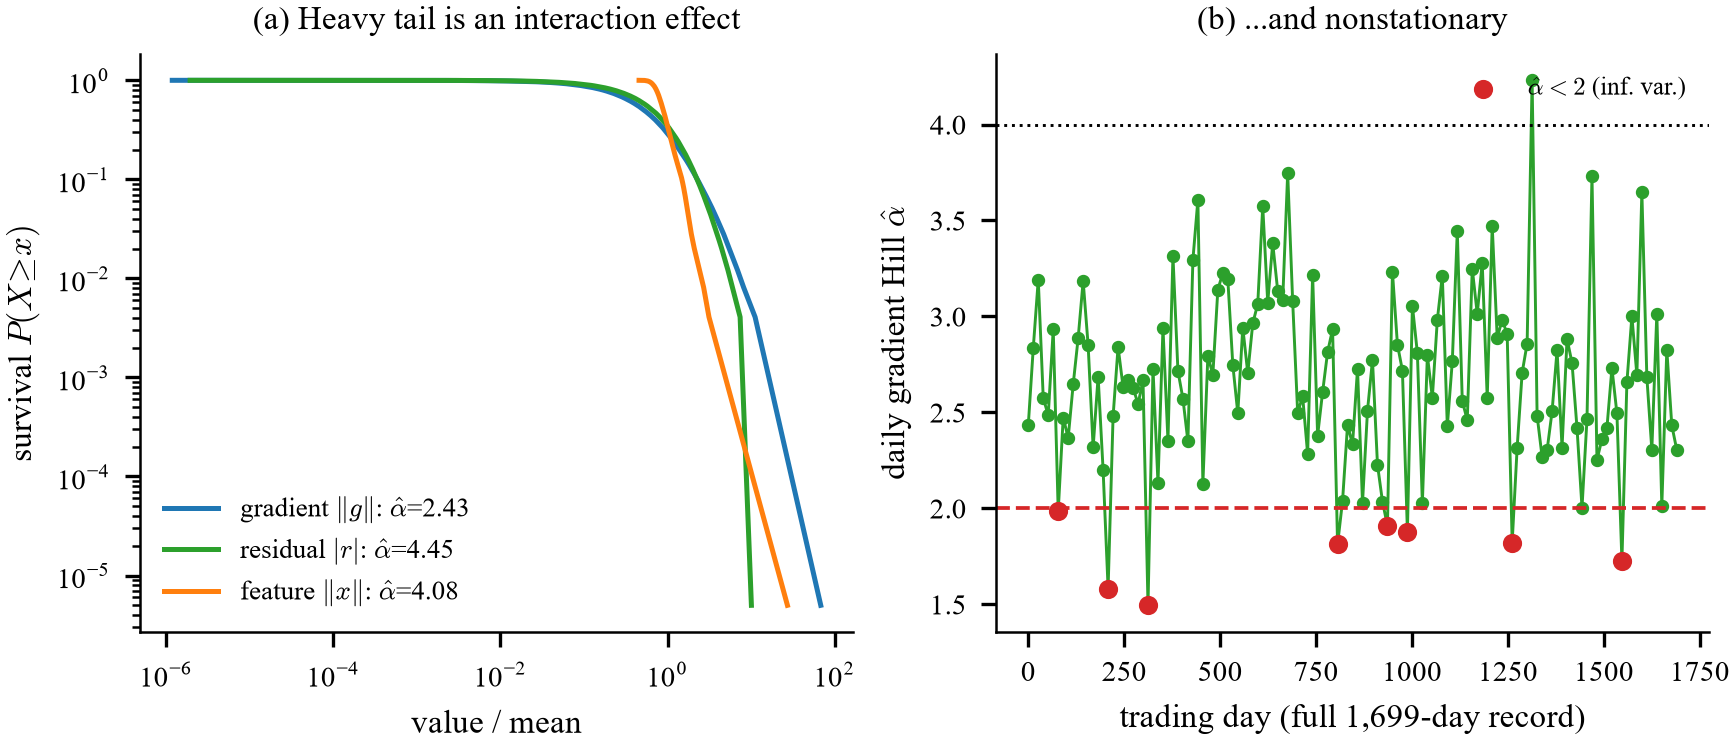
\includegraphics[width=\textwidth]{fig1_problem.png}
\caption{\textbf{The phenomenon: an \emph{interaction} tail, on a scale that drifts}
(\cref{sec:experiments}). (a)~The \emph{pooled} gradient tail (Hill $\hat\alpha\approx2.43$) is
heavier than either its residual or its feature factor ($\hat\alpha\approx4$), because extreme
features and residuals co-occur. (b)~The daily gradient tail index drifts across the full
$1{,}699$-day record; the per-day dips below $2$ are noisy single-day Hill estimates and we do
not rely on them (\cref{app:tables}).}
\label{fig:problem}
\end{figure*}

\begin{figure*}[t]
\centering
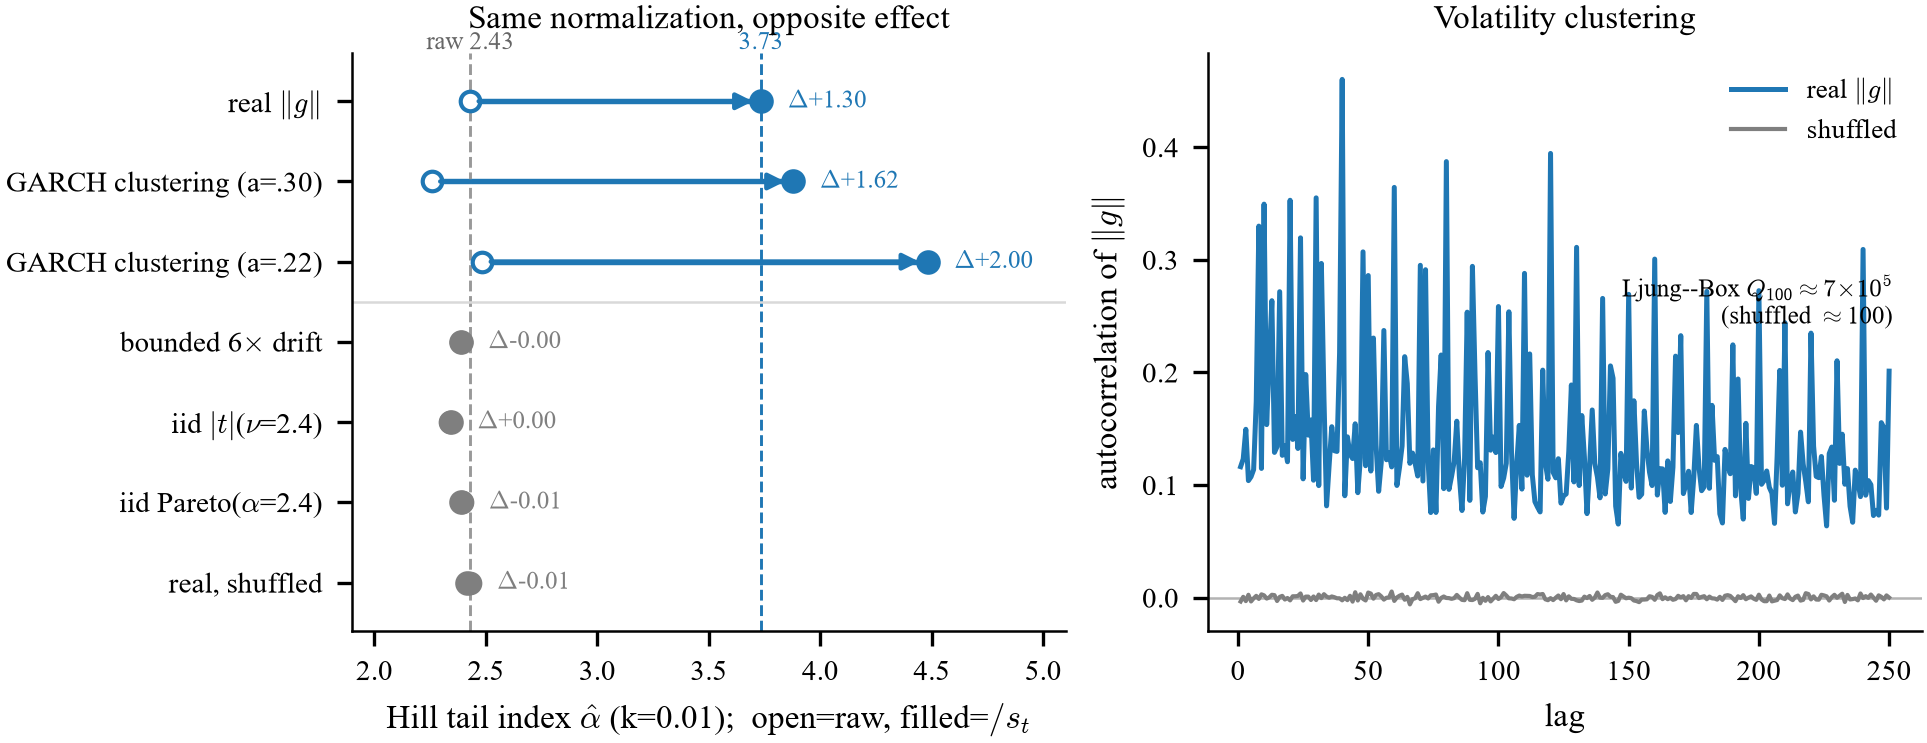
\includegraphics[width=0.9\textwidth]{fig7_nullcontrol.png}
\caption{\textbf{The lightening is removability, not manufacture} (\cref{sec:experiments}).
(a)~Hill index before (open) and after (filled) causal scale-normalization, $k{=}0.01$. The
\emph{same} operation lightens the real gradient tail ($2.43\!\to\!3.73$) and a
light-innovation GARCH surrogate, but leaves an order-\emph{shuffle}, iid heavy streams of
known index, and a bounded $6\times$ drift essentially unchanged ($\Delta\!\approx\!0$): what
is removed is serial dependence, not the marginal, and it is no estimator artifact.
(b)~Rank autocorrelation of $\norm{\gt}$ decays slowly---the volatility clustering the tracker
exploits---and vanishes under shuffling.}
\label{fig:nullcontrol}
\end{figure*}

\paragraph{Scale-free updates dominate scale-dependent ones.} Streaming one learner
through the multi-regime window and sweeping the learning rate
(\cref{tab:jane,fig:main}), the methods split cleanly by whether their step responds to the
gradient \emph{scale}. \emph{Scale-dependent} methods---plain OGD and the robust clippers
(AdaptiveClip, RobustOMD), whose threshold $\tau_t=c\,s_t$ rescales with the regime---are
fragile: they stay bounded only to $\mathrm{lr}\approx10^{-2}$ and reach best
$R^2\approx0.01$--$0.14$, because any larger rate diverges when the scale spikes
(\cref{fig:mechanism}).

The \emph{scale-free} family---normalized-GD, SN-OMD, uncapped scale-adaptive OGD, the
fixed-$\tau$ clip, and AdaGrad-Norm, none of whose step bounds move with the regime---stays
bounded far higher and reaches $R^2\approx0.08$--$0.38$ across the two protocols. Batching to
per-step does not manufacture SN-OMD's accuracy: aggregating the $\sim\!9$ correlated symbols
of a step leaves SN-OMD essentially unchanged ($0.285\!\to\!0.307$), so no contemporaneous
cross-sectional information is in play, while it lifts fragile OGD without fixing it and
\emph{halves} the uncapped endpoint (\cref{tab:jane}).

\paragraph{What the tracked scale and the cap buy---and what they do not.}
A whole \emph{family} of \emph{bounded} scale-free updates---the list above minus the
\emph{uncapped} endpoint, which is scale-free but carries no bound at all: SN-OMD,
normalized-GD, the fixed-$\tau$ clip, and AdaGrad-Norm---closes the accuracy gap to the
divergent baselines, and \emph{no single member dominates}. On the reported window the two top
entries use \emph{neither} a tracked scale nor a cap (fixed-$\tau$ clip per-step, AdaGrad-Norm
per-row), but neither ranking survives replication (\cref{tab:replication} below): the winner
differs by protocol and no member leads on both, so what earns the gain is \emph{normalization
in general}---any bounded scale-free step---of which SN-OMD is one instance. The family is not homogeneous, though:
useful learning-rate ranges span two orders of magnitude across its members
(\cref{tab:jane}), so ``bounded scale-free'' is necessary for stability while the \emph{ceiling}
depends on how the step behaves \emph{within} the bound.

What singles out SN-OMD is therefore two things, not uniform accuracy. \emph{(i) Predictability:} its scale $s_t$ is a
\emph{predictable} tracker, which makes the dynamic-regret bound (\cref{thm:regretbody}) go
through---normalized-GD's instantaneous $1/\norm{\gt}$ is not predictable and discards
magnitude every round. One \emph{predictable} instance, the block-median scale, also delivers
\emph{co-leading} per-row accuracy: paired across the ten windows it beats every baseline it
does not tie, and it \emph{ties} the normalize-and-clip baseline at the top---on this one
protocol only (intervals and window counts in \cref{app:tracker}). The two claims are
distinct: \cref{thm:regretbody} needs predictability, which says nothing about how accurate any
particular predictable tracker is, so the block median's co-lead is a property of \emph{that}
tracker (\cref{sec:tracker}), not of predictability.

\emph{(ii) The cap.} A finite $M$ bounds the step directly, but non-divergence is not unique
to it: AdaGrad-Norm stays bounded to a \emph{wider} $\mathrm{lr}\le10$ with no cap. What the cap
distinctly buys is an interior accuracy optimum (\cref{sec:msweep})---\emph{sharp} when the
normalized tail is heavy, \emph{broad} when it is mild, as on Jane: there a finite cap still
beats full normalization by ${+}0.11$ per-row, though the mid-range caps sit within noise.

\paragraph{Replication across ten disjoint windows.} A single contiguous window cannot
settle a claim that is \emph{about} regime dependence, so we re-run the entire comparison on
\emph{ten} disjoint $150{,}000$-row windows spanning the full $1{,}699$-day record, with every
method's hyperparameters \emph{frozen} at its window-1 tuning---the realistic
tune-once-then-deploy setting (\cref{tab:replication}). Two findings are sharp. \emph{(i) The
stability partition replicates and hardens:} every finite-cap bounded scale-free method stays
bounded on all ten windows ($0/10$ divergences), while the uncapped $M\!\to\!\infty$ endpoint
diverges on $7/10$ (per-row) and plain OGD's frozen rate diverges on $9/10$ (per-step). The
uncapped endpoint's $0/10$ per-step is not batching conferring robustness but a lower frozen
rate ($\mathrm{lr}{=}0.2$ vs.\ $0.5$ per-row), so it underfits ($0.10\!\pm\!.02$) instead of
diverging; the finite cap is stable at every rate on \emph{both} protocols. Both halves of the
stability claim therefore hold across the whole record, not merely on the reported window.

\emph{(ii) No bounded member dominates, and which one is best is tracker- and
protocol-dependent.} Per-row two methods co-lead in a statistical
tie---the block-median SN-OMD ($0.28\!\pm\!0.09$) and the normalize-and-clip baseline of
\citet{cutkoskymehta2021} ($0.29\!\pm\!0.04$; the paired contrast of \cref{app:tracker}---%
$+0.004$, CI $[-0.014,+0.023]$, $6/10$---predates the cap
tuning)---both clear of the rest (fixed-$\tau$ $0.21$,
AdaGrad-Norm $0.20$, normalized-GD $0.18$), among which the per-window winner rotates between the
clip and AdaGrad. Per-step the ordering reshuffles without separating the pack (block $0.24$,
SN-OMD $0.21$, clip $0.20$, AdaGrad-Norm $0.19$, all within one standard deviation); normalized-GD and CM collapse to $0.09\!\pm\!0.21$,
their window-1-optimal rates having overfit that window (\cref{app:grid}). The block median buys ${\approx}{+}0.04$ of per-row mean over the
deployed EMA at the cost of spread ($\pm.09$ vs.\ $\pm.05$), neither row going negative on any
window, so the tracker choice trades accuracy against variability rather than dominating---and
the more accurate tracker is the one \emph{without} a proven $W_s$ bound
(\cref{sec:tracker,app:tracker}).

\begin{table}[t]
\caption{\textbf{Ten-window replication, hyperparameters frozen from window~1}
(\cref{sec:experiments}; ten disjoint $150$k-row windows across the $1{,}699$-day record).
Mean$\pm$std weighted $R^2$ and divergence count (a method ``diverges'' if its peak rolling loss
blows up at the frozen rate). Every finite-cap bounded scale-free method stays bounded on all ten
windows; the uncapped endpoint and plain OGD do not, and \emph{no single member dominates across
both protocols} (\cref{sec:experiments,app:tracker}). Each method is tuned over its own free
parameters: both SN-OMD rows over $(\mathrm{lr},M)$, the same two-parameter budget fixed-$\tau$
gets over $(\mathrm{lr},\tau)$, and the threshold-free methods over $\mathrm{lr}$ alone---their
whole parameter space. Every selected optimum is interior except the per-step SN-OMD row, which
pins at both grid edges (\cref{app:grid}). CM at $\beta{=}0$ \emph{is} normalized-GD, so their
per-step cells are bit-identical rather than duplicated.}
\label{tab:replication}
\centering
\begin{small}
\setlength{\tabcolsep}{3.5pt}
\begin{tabular}{lcccc}
\toprule
 & \multicolumn{2}{c}{per-row} & \multicolumn{2}{c}{per-step} \\
\cmidrule(lr){2-3}\cmidrule(lr){4-5}
Method & mean$\pm$std & div & mean$\pm$std & div \\
\midrule
OGD                                    & $0.00\pm.04$ & $0/10$ & --- & $9/10$ \\
Scale-adaptive OGD ($M\!\to\!\infty$)  & --- & $7/10$ & $0.10\pm.02$ & $0/10$ \\
Normalized-GD ($M\!\to\!0$)            & $0.18\pm.03$ & $0/10$ & $0.09\pm.21$ & $0/10$ \\
Fixed-$\tau$ clip                      & $0.21\pm.03$ & $0/10$ & $0.20\pm.13$ & $0/10$ \\
AdaGrad-Norm                           & $0.20\pm.07$ & $0/10$ & $0.19\pm.03$ & $0/10$ \\
Cutkosky--Mehta (2021)                 & $\mathbf{0.29}\pm.04$ & $0/10$ & $0.09\pm.21$ & $0/10$ \\
\textbf{SN-OMD ($M$ tuned, ours)}      & $0.24\pm.05$ & $0/10$ & $0.21\pm.12$ & $0/10$ \\
\quad\emph{+ block-median tracker}     & $0.28\pm.09$ & $0/10$ & $\mathbf{0.24}\pm.11$ & $0/10$ \\
\bottomrule
\end{tabular}
\end{small}
\end{table}

\paragraph{Negative control.} If the advantage is really about scale drift, it should
vanish when the scale is constant. Imposing genuine stationarity in the synthetic harness
($\sigma_t\equiv1$, $p{=}2$, static reachable comparator---the one stream where
stationarity can be enforced), tuned SN-OMD is if anything \emph{worse} than tuned OGD
(steady excess loss $6.4$ vs.\ $5.5\!\times\!10^{-4}$ over $400$ seeds, a $16\%$ gap the
wrong way; both rates interior on their grids, \cref{app:grid}): the advantage disappears as the thesis
predicts (a $100\mathrm{k}$-row Jane slice is \emph{not} a valid stationarity control---it
still has $\sim30\%$ within-day drift---so its lead there is expected).

\paragraph{Further experiments (deferred to \cref{app:further}).} Two supporting studies
develop (i)~the \emph{cap frontier}---an $M$-sweep across the interpolation from normalized-GD
($M\to0$) to uncapped scale-adaptive OGD ($M\to\infty$), with a \emph{sharp} interior optimum
under an imposed heavy tail and a \emph{broad} one on Jane; and (ii)~the empirical discharge of
\cref{ass:track}, which measures $W_s$ growing \emph{linearly} in $T$---the reason
\cref{thm:regretbody}'s rate is per-regime.

\section{Related Work}
\label{sec:related}

\paragraph{Scale mixtures and volatility models.} That a drifting scale makes
conditionally light-tailed data look unconditionally heavy-tailed is classical \emph{for
asset returns}: Clark's subordinated-process model \citep{clark1973}, the ARCH/GARCH family
\citep{engle1982,bollerslev1986}, and the finding that returns \emph{standardized by
realized volatility} are approximately Gaussian \citep{andersen2001}. Our
pooled-vs-normalized separation is the same phenomenon; we claim no novelty for the
mechanism. What is new is (i) that it holds for the \emph{loss gradients} of an online
learner---so it governs \emph{optimization}, not just modeling; (ii) that the gradient's
heavy tail is an \emph{interaction} effect (feature $\times$ residual co-movement), heavier
than either factor alone (\cref{fig:problem}); and (iii) the algorithm-design
consequence---the scale-normalized update and its cap-interpolation frontier
(\cref{sec:msweep})---which the volatility literature does not address.

\paragraph{Robust estimation and clipping.} Robust estimators (Catoni, median-of-means,
trimmed mean) achieve sub-Gaussian deviations under a finite variance
\citep{catoni2012,devroye2016,lugosi2019}, imported into sequential decision-making by
\citet{bubeck2013}; in optimization, gradient clipping yields high-probability convergence
under heavy-tailed noise \citep{zhang2020clip,gorbunov2020,nguyen2023}. Closest to ours,
\citet{cutkoskymehta2021} \emph{normalize and clip} for high-probability non-convex
convergence under $\mathbb{E}\norm{\gt}^p\!<\!\infty$; we differ in normalizing by a
\emph{predictable} tracked scale (not a fixed clip of the current gradient) and in targeting
\emph{dynamic} regret under a \emph{drifting} scale rather than static convergence.

We ran their method head-to-head across the ten frozen windows, tuned over its momentum
coefficient. It stays bounded ($0/10$) and \emph{co-leads} per-row, statistically tied with the block-median
SN-OMD (\cref{tab:replication,app:tracker}). That co-lead is bought by \emph{momentum}, not the
clip: at $\beta{=}0$ CM reduces exactly to normalized-GD, and its per-row edge over it is almost
all the $\beta{=}0.5$ momentum term, the clip idle on its plateau (\cref{app:tracker,tab:grid}).
So momentum-normalized SGD, not clip-plus-normalization, ties the tracked scale, and neither
leads both protocols; what the \emph{predictable} scale adds is the dynamic-regret guarantee,
not a measured accuracy edge.

\paragraph{Heavy-tailed online learning.} \citet{liu2026oco} show plain OGD is optimal
\emph{in expectation} on a bounded domain, and \citet{zhangcutkosky2022} give parameter-free
\emph{high-probability} static regret $\tilde O(\norm u T^{1/p})$ over unbounded domains,
whose central obstacle---exponentially large iterates---our cap sidesteps. Both are static;
the dynamic, nonstationary regime we target sits outside them, and our budget heuristic
(\cref{sec:lower}) suggests why it is harder (a proper $P_T$-constrained lower bound remains
open). Concurrently, \citet{aggarwal2026dynamic} attain parameter-free \emph{universal
dynamic} regret under heavy tails \emph{in expectation}, via restarted-AdaGrad experts with
a Hedge meta-algorithm and no clipping; we differ in targeting a \emph{drifting scale}
through a predictable tracker and a hard cap, and in a \emph{high-probability} (not
in-expectation) guarantee.

A concurrent line sharpens the normalization-versus-clipping question for \emph{offline
non-convex} SGD, proving normalization---with or without clipping---suffices for convergence
under only a bounded $p$-th moment \citep{liuzhou2025nonconvex,hubler2025clipping,sun2024normalization}; we instead
target \emph{online dynamic regret} under a \emph{drifting} scale, and add the measurement that
the gradient tail is itself a predictable-scale artifact.

\paragraph{Dynamic, scale-free, and adaptive OL.} Dynamic regret against a moving comparator
goes back to \citet{zinkevich2003}; normalized and scale-free methods adapt to an unknown
gradient scale \citep{levy2017,orabona2018}; strongly-adaptive and parameter-free wrappers adapt to unknown
interval/regime structure \citep{daniely2015,cutkosky2020}, which we use as a black box to
remove knowledge of the regime length.

\paragraph{Adaptive optimizers.} Coordinate-wise adaptive methods (AdaGrad, RMSProp, Adam)
also rescale by a running second moment. We ran RMSProp and Adam head-to-head rather than
reasoning about them, which corrected an argument we had made from the armchair
(\cref{app:adaptive}): their EMA denominator \emph{bounds} the step rather than inflating it, so
they do not diverge, and they \emph{tie} SN-OMD once the step schedule is matched---the fourfold
gap a naive comparison shows is the schedule, not the preconditioner. They belong in the bounded
family; what they lack, like \emph{AdaGrad-Norm} ($0.20\!\pm\!.07$ per-row;
\cref{tab:replication}), is a \emph{predictable} scale and the dynamic-regret guarantee
(\cref{thm:regretbody}).

\section{Conclusion}
\label{sec:conclusion}

On real streams the difficulty is a strongly \emph{nonstationary} gradient scale whose
\emph{predictable} part the learner faces: the pooled gradient looks heavy-tailed (volatility
clustering of a heavy-tailed conditional scale) while the causally normalized gradient is much
lighter. SN-OMD normalizes and caps at a scale-free constant, so its iterates provably cannot
diverge ($O(\sqrt t)$ for any rate) and attain $T^{1/p}$ \emph{per regime}; across ten frozen
windows the \emph{bounded scale-free} family stays bounded where OGD and scale-dependent clipping
diverge, and what singles out SN-OMD is a \emph{predictable} tracker---not an accuracy win: with
the block-median scale it co-leads per-row.

\paragraph{Limitations.} SN-OMD is not fully tuning-free: the rate is setting-dependent, and
\cref{tab:replication} tunes the cap $M$ alongside it, so the deployed method carries \emph{two}
tuned parameters (the tracker's decay and winsorization are left untuned). The $W_s=O(V_\sigma^+)$ guarantee covers only the two-timescale envelope
(\cref{ass:track}), not the deployed EMA/block-median trackers (empirical only,
\cref{sec:tracker}). Our
\emph{positive} evidence is from two financial streams, with the MNIST probe a negative boundary
(\cref{app:secondmarket}), so the mechanism is domain-general in principle but validated on
markets only. Finally, the normalized residual tail is dominated by
\emph{causal-estimation cost} ($\hat\alpha\approx3.73$; \cref{tab:residual}), so with $p>2$ the
cap is for stability alone.

\section*{Ethics Statement}
This work studies online prediction on public financial-market and cryptocurrency data and
poses no direct ethical concerns: it uses no human-subjects data, no personally identifying
information, and the datasets are publicly released for research (the Jane Street Kaggle
competition and public Binance BTC/USDT bars). Deployed trading systems built on any online
learner can amplify market instability; our contribution is a \emph{stability} guarantee that,
if anything, bounds rather than amplifies runaway behavior, and we make no claim of profitable
trading. This statement is optional under the ICLR Code of Ethics and does not count toward the
page limit.

\section*{Reproducibility Statement}
All theoretical claims are stated with their assumptions in \cref{sec:problem,sec:method} and
proved in \cref{app:regret,app:proofs}. The code supplement (\S Software and Data) provides the
learner, scale trackers, configs, and a script for every figure and number; the synthetic and
tail-index results are runnable without any market data, and a deterministic test suite plus a
SHA-pinned headline input guard against drift. The Jane Street and crypto numbers require the
public competition data (Kaggle-gated), as disclosed in \cref{sec:experiments}. The headline
market numbers are deterministic---a single streaming pass over the pinned input, with no
seed averaging---so their reported uncertainty comes only from the seeded block bootstrap
(\cref{tab:jane}, \cref{sec:tracker}) and, for the synthetic experiments, the stated seed
counts (e.g.\ the $400$-seed and five-seed runs). All experiments run on a single commodity
CPU with no accelerator required: the only neural component (MNIST-CNN gradient norms,
\cref{app:secondmarket}) trains a small network that runs on CPU and is cached, so the full
figure-and-table suite reproduces without a GPU.

\section*{Use of Large Language Models}
Large language models were used as assistive tools during this project: for prose editing and
LaTeX formatting; for code refactoring and documentation; for related-work search and
cross-checking; for feedback on experimental methodology and analysis; and for an independent
audit pass over the manuscript that assisted in checking the theorem derivations and
paper--code consistency,
and assisted the preparation of the submission in the ICLR format. LLMs were \emph{not} used to generate experimental data and did not originate the
core research question, the theoretical results, or the empirical findings; every theorem,
proof, experimental design, and reported number was verified by the authors, who take full
responsibility for the content. This statement does not count toward the page limit.

\bibliographystyle{iclr2027_conference}
\bibliography{refs}

\newpage
\appendix

\section*{Software and Data}
The accompanying anonymized code provides the \texttt{ScaleNormalizedOGD} learner---named for
the projected-gradient form the mirror step takes under the Euclidean regularizer
(\cref{sec:method}), so it implements \cref{alg:snomd} exactly---the scale trackers
(winsorized EMA, two-timescale envelope, block median), the configs, and the scripts that
reproduce every figure and number, including \cref{tab:residual}'s real-data rows
(\texttt{research\_review2\_checks.py}) and its GARCH-surrogate rows
(\texttt{research\_residual\_surrogate.py}, fully synthetic---runnable without any market data).
Data: the public Jane Street Real-Time Market Data Forecasting competition, Binance BTC/USDT
hourly bars, and MNIST-CNN gradient norms (the latter two in \cref{app:secondmarket}).

\section{Additional experimental tables and figures}
\label{app:tables}
Collected here for space, all of it \emph{single-window} material: the residual tail-index
decomposition (\cref{tab:residual}), the leakage controls (\cref{tab:leakage}), the tuned
method comparison (\cref{tab:jane}), the learning-rate sweep behind it (\cref{fig:main}), and
the scale-drift/clipping mechanism figure (\cref{fig:mechanism}). The ten-window replication
(\cref{tab:replication}) and its reading remain in the body, since the across-window
numbers---not the single-window tuning---carry the accuracy claims.

\paragraph{Tail diagnostics in detail (\cref{tab:residual}).} The tail indices of
\cref{sec:experiments} are Hill estimates on gradients at the fixed optimum $w^\star$: the
pooled index from ${\sim}200{,}000$ gradients, the daily-drift index from the full record.
Causal normalization lightens the pooled $\hat\alpha\approx2.43$ to $\approx3.7$ (the deployed
causal winsorized-EMA $s_t$), $\approx3.2$ (non-causal median), or $\approx2.9$ (trailing
median), and the lightening is positive at every threshold and estimator (\cref{tab:residual}).
What remains is dominated by \emph{causal-estimation cost} rather than by a resolvable residual
tail: the \emph{same} estimator run non-causally recovers only $\sim\!+0.3$, while on a GARCH
surrogate with Gaussian innovations---\emph{zero} residual tail by construction---the same
causal tracker still reads $\hat\alpha\approx3.9$--$4.8$, the spread running over both the
threshold $k$ and the assumed persistence, against a true-$\sigma_t$ oracle of $\approx8$--$10$
(\cref{tab:residual}). The real $3.73$ sits just \emph{below} that zero-residual band, by about the
surrogate's own sensitivity to its persistence, so we cannot separate a genuine residual
conditional tail from a scale merely less predictable than GARCH(1,1); either way the residual
is dominated by estimation cost and $\hat\alpha\approx3.7$ leaves $p>2$. The serial dependence
the tracker exploits is strong and long-ranged: rank (Spearman) autocorrelation
$\approx0.16$ at lag $100$ and rank-based Ljung--Box $Q_{100}\approx7\!\times\!10^{5}$ (ranks
are bounded, so the $\chi^2$ is valid; a shuffled control gives $\approx116$). The three null
controls of \cref{fig:nullcontrol}---order-shuffle, iid streams of known index, and the
light-innovation GARCH surrogate---are produced by
\texttt{research\_null\_normalization.py} in the anonymized supplement. The shuffle control
leaves the \emph{pooled} index exactly unchanged---an order-statistic identity, since a
permutation does not touch the marginal---while abolishing the lightening, which is what makes
it decisive. Finally, per-day
$\hat\alpha$ dips below $2$ on a minority of days, but single-day Hill estimates are noisy and
we do not rely on them; the per-regime budget heuristic of \cref{sec:lower} rests on exactly
those days, which is why we keep it qualitative.

\paragraph{Why one method can appear at two rates (\cref{tab:jane}).} Every method is
reported at \emph{its own} tuned rate, so the same method can carry different rates in
different experiments. Normalized-GD's per-row optimum is $\mathrm{lr}{=}3$ on the baseline
grid used for \cref{tab:jane} ($0.220\!\pm\!.037$), and $\mathrm{lr}{=}2$ on the cap-frontier
grid where it is the $M\!\to\!0$ endpoint ($0.197\!\pm\!.024$; \cref{sec:msweep}). Both are
that experiment's own optimum, not a duplicated or stale row. \cref{tab:jane} is
interpreted in \cref{sec:experiments}, and its block-median tracker variant in
\cref{sec:tracker}.

\paragraph{Leakage controls in detail (\cref{tab:leakage}).} Permuting the $(y_t,\omega_t)$
pairs drives every method to $R^2\le0$ (SN-OMD $-0.00$), so there is no label leakage. A static
weighted ridge with \emph{full} look-ahead reaches only $0.02$ and a per-day look-ahead oracle
$0.18$, both below online SN-OMD's $0.28$: the accuracy is carried by fast within-day adaptation
that no fixed-partition linear oracle matches. And the weights learned on this window, applied
unchanged to a disjoint later window, give $R^2=-1.7$, whereas that window's own prequential run
gives $+0.22$---the score is tracking, not transfer.

\begin{table}[htbp]
\caption{\textbf{The lightening is order-one and estimator-stable; the residual is
causal-estimation cost} (\cref{sec:experiments}). Hill $\hat\alpha$ of the normalized
$\norm{\gt}$ at three tail fractions $k$ (larger $=$ lighter). The deployed causal tracker
lightens the raw pooled tail by $+1.0$ to $+1.5$; the \emph{same} estimator run non-causally adds
only $\sim\!+0.3$. The GARCH surrogate (Gaussian innovations, \emph{zero} residual tail,
calibrated to the real raw index) reads $\hat\alpha\approx4.1$--$4.8$ after the same causal
tracking ($\approx3.9$ at lower persistence; \cref{fig:nullcontrol}) against a true-$\sigma_t$
oracle of $\approx8$--$10$: causal estimation \emph{alone} costs several index points. The real
$3.73$ sits \emph{just below} this zero-residual band, so the residual is dominated by
causal-estimation cost and the $(1,2]$ apparatus does not bind here.}
\label{tab:residual}
\centering
\begin{small}
\setlength{\tabcolsep}{5pt}
\begin{tabular}{lccc}
\toprule
Normalization of $\norm{\gt}$ & $k{=}.005$ & $k{=}.01$ & $k{=}.02$ \\
\midrule
\multicolumn{4}{l}{\emph{Real gradient stream:}}\\
raw pooled (none)                        & $2.55$ & $2.43$ & $2.32$ \\
causal winsorized-EMA \emph{(deployed)}  & $4.02$ & $3.73$ & $3.36$ \\
\quad centered EMA (non-causal twin)     & $4.16$ & $4.05$ & $3.58$ \\
trailing median (causal)                 & $3.24$ & $2.87$ & $2.60$ \\
\quad centered median (non-causal)       & $3.62$ & $3.18$ & $2.81$ \\
\midrule
\multicolumn{4}{l}{\emph{GARCH surrogate (Gaussian innov.; zero residual tail):}}\\
raw pooled (none)                        & $2.54$ & $2.48$ & $2.44$ \\
causal winsorized-EMA                    & $4.81$ & $4.48$ & $4.08$ \\
\quad true-$\sigma_t$ oracle             & $10.3$ & $9.05$ & $7.75$ \\
\bottomrule
\end{tabular}
\end{small}
\end{table}

\begin{table}[htbp]
\caption{\textbf{Leakage controls for the prequential $R^2$} (\cref{sec:experiments};
date$[0,120)$, $150$k rows, causal standardization). The headline $R^2\approx0.28$ survives a shuffled-label null and is
not a look-ahead artifact: it comes from within-day adaptation on a nonstationary stream, not
from seeing the target or a transferable static fit.}
\label{tab:leakage}
\centering
\begin{small}
\begin{tabular}{lcc}
\toprule
Control & $R^2$ & Reads as \\
\midrule
Shuffled label (perm.\ $y$)               & $-0.00$     & no label leakage \\
Offline ridge (static\,/\,per-day oracle) & $0.02/0.18$ & online $0.28$: adaptation \\
Frozen $w_T$, forward window              & $-1.7$      & tracking, not transfer \\
\bottomrule
\end{tabular}
\end{small}
\end{table}

\begin{table}[htbp]
\caption{\textbf{Single-window tuned comparison} (\cref{sec:experiments}; continuous Jane
Street stream, \emph{causal} standardization, both granularities). Best weighted $R^2$ with
each method at its own tuned rate, and its largest stable rate; each $R^2$ carries $\pm$one
circular block-bootstrap standard error (block $\approx$ one trading day, $4000$ resamples).
Scale-\emph{dependent} methods (top) are fragile, stable only to
$\mathrm{lr}\!\approx\!10^{-2}$; the \emph{bounded scale-free} family (bottom)---SN-OMD,
normalized-GD, a fixed-$\tau$ clip ($\tau{=}20$) and AdaGrad-Norm, all satisfying
\cref{thm:stability}---stays bounded far higher and is far more accurate, with \emph{none}
dominating. These are one window's numbers, and the per-protocol leaders here (fixed-$\tau$
clip per-step, AdaGrad-Norm per-row) do \emph{not} carry over as unique leaders across windows
(\cref{tab:replication}). $R^2$ is not comparable to competition scores.}
\label{tab:jane}
\centering
\begin{small}
\setlength{\tabcolsep}{3.5pt}
\begin{tabular}{lccc}
\toprule
Method & $R^2$ per-row & $R^2$ per-step & Stable lr \\
\midrule
\multicolumn{4}{l}{\emph{Scale-dependent (fragile):}}\\
OGD                                  & $0.018{\scriptscriptstyle\pm.006}$ & $0.139{\scriptscriptstyle\pm.012}$ & $\le 10^{-2}$ \\
AdaptiveClip / RobustOMD             & $\sim0.01$ & --- & $\le 10^{-2}$ \\
\midrule
\multicolumn{4}{l}{\emph{Scale-invariant (bounded; stable lr per row):}}\\
Normalized-GD ($M\!\to\!0$)          & $0.220{\scriptscriptstyle\pm.037}$ & $0.371{\scriptscriptstyle\pm.077}$ & $\le 5$ \\
Scale-adaptive OGD ($M\!\to\!\infty$)& $0.159{\scriptscriptstyle\pm.024}$ & $0.080{\scriptscriptstyle\pm.013}$ & $\le 1$ \\
Fixed-$\tau$ clip (const $M$)        & $0.246{\scriptscriptstyle\pm.046}$ & $\mathbf{0.382}{\scriptscriptstyle\pm.047}$ & $\le 0.2$ \\
AdaGrad-Norm                         & $\mathbf{0.329}{\scriptscriptstyle\pm.030}$ & $0.219{\scriptscriptstyle\pm.014}$ & $\le 10$ \\
\textbf{SN-OMD ($M{=}5$, ours)}      & $0.285{\scriptscriptstyle\pm.080}$ & $0.307{\scriptscriptstyle\pm.059}$ & $\le 2$ \\
\bottomrule
\end{tabular}
\end{small}
\end{table}

\begin{figure*}[t]
\centering
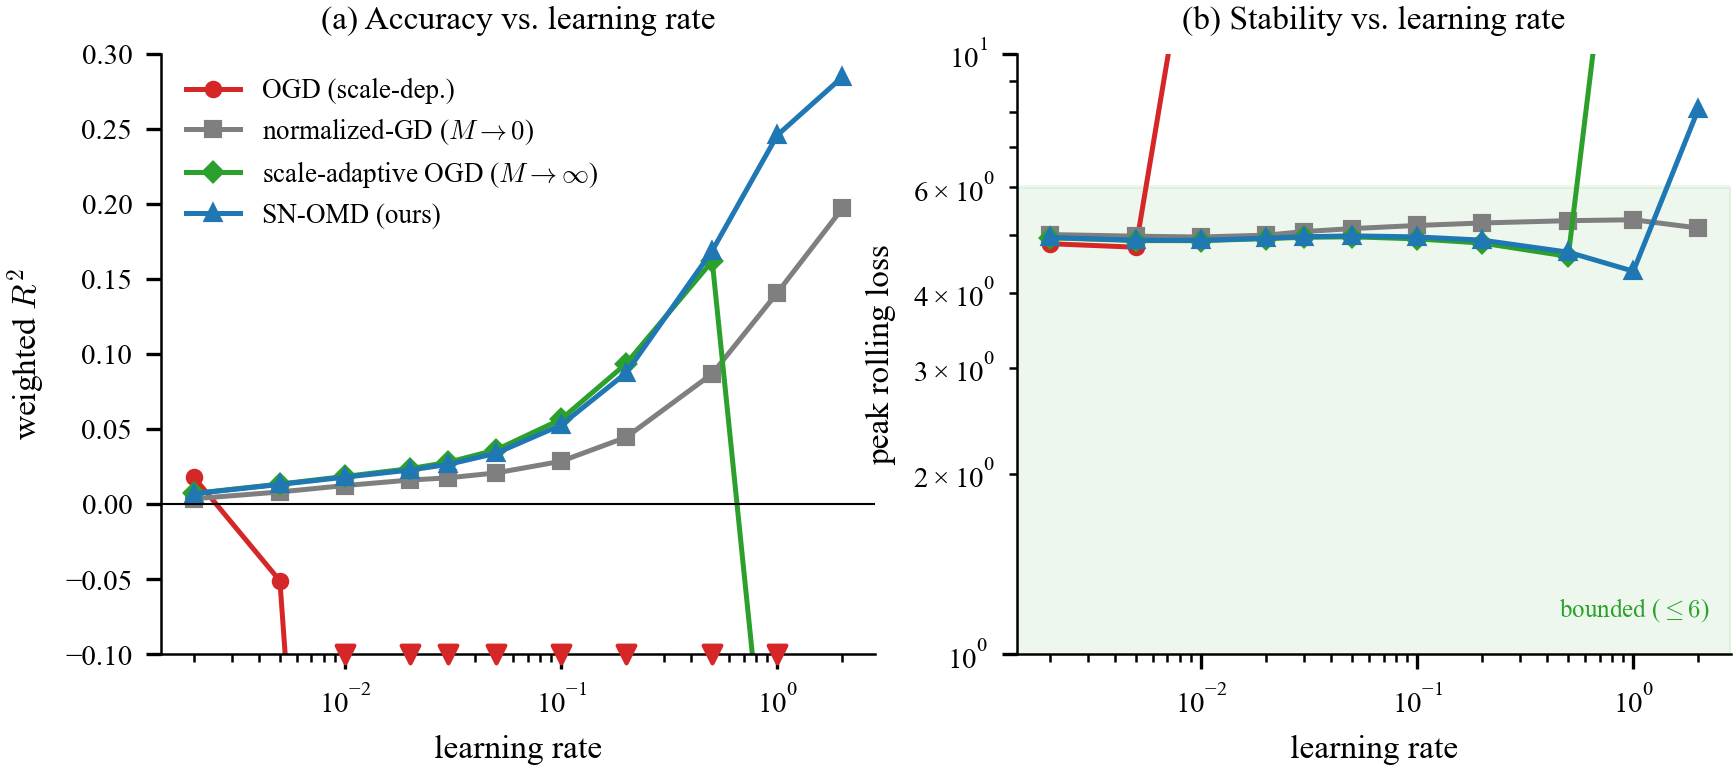
\includegraphics[width=0.9\textwidth]{fig3_main.png}
\caption{\textbf{The stability dichotomy on the reported window} (continuous multi-regime
stream, \emph{causal} standardization, per-row; the across-window version is
\cref{tab:replication}). The cap family: OGD (scale-dependent) against the $M\!\to\!0$
endpoint (normalized-GD), the $M\!\to\!\infty$ endpoint (uncapped scale-adaptive OGD), and
SN-OMD ($M{=}5$). (a)~Weighted $R^2$ vs.\ learning rate: OGD cliffs above
$\mathrm{lr}{=}10^{-2}$ (off-scale) and the uncapped endpoint diverges at large rates, while
the scale-free methods climb to $R^2\approx0.2$--$0.3$ with overlapping intervals
(\cref{tab:jane}). (b)~Peak rolling loss: the two scale-dependent curves explode
($10^2$--$10^{30}$); normalized-GD ($\approx5$) and SN-OMD ($\approx8$ at its top stable
$\mathrm{lr}{=}2$) stay single-digit.}
\label{fig:main}
\end{figure*}

\begin{figure}[htbp]
\centering
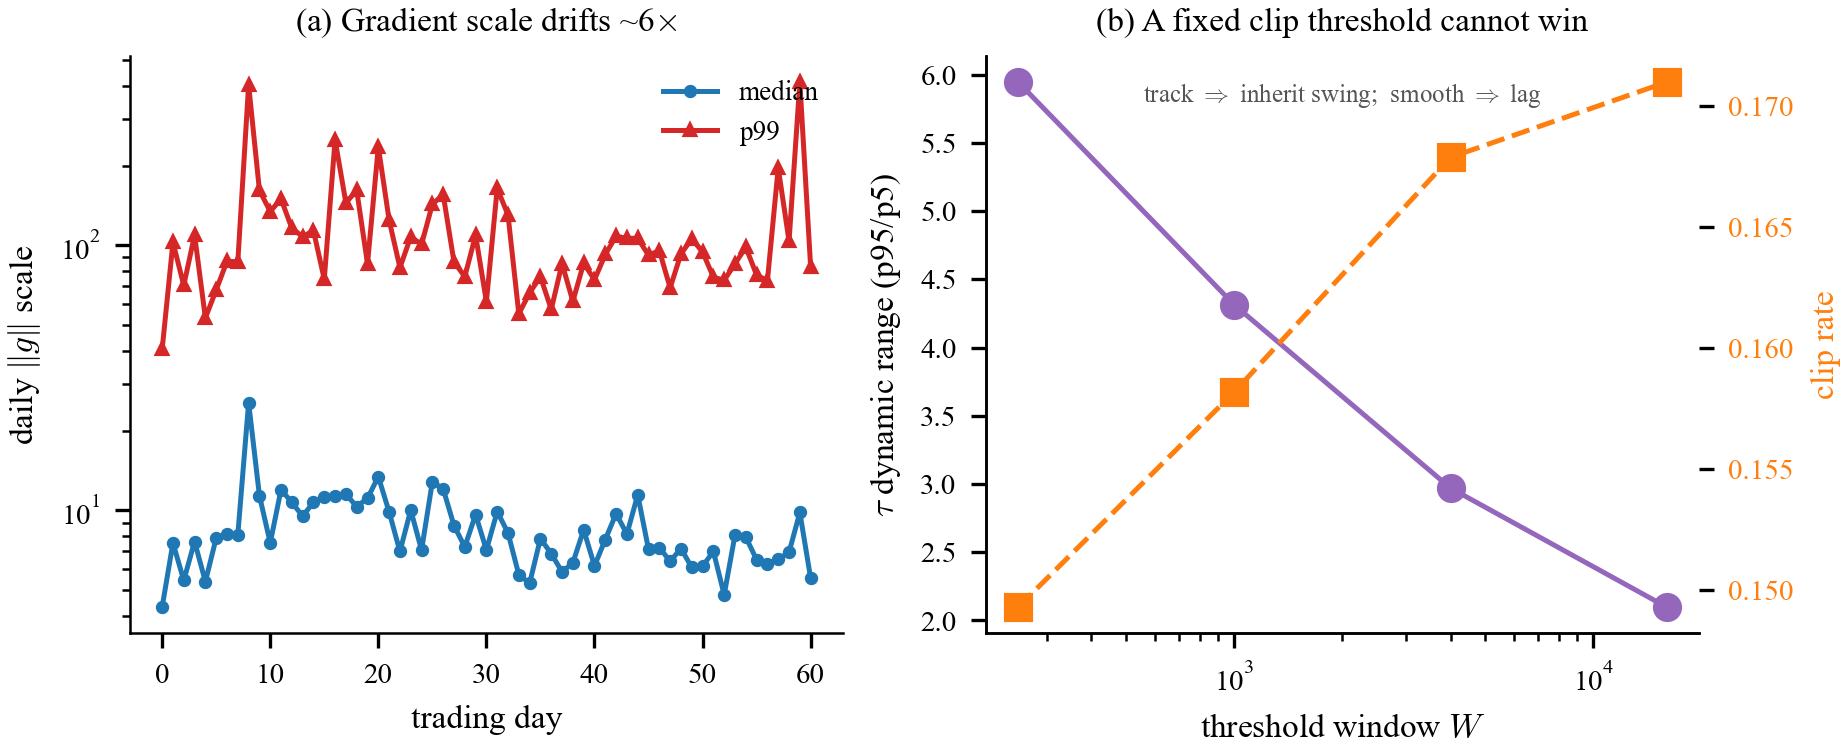
\includegraphics[width=\columnwidth]{fig2_mechanism.png}
\caption{\textbf{Why scale-dependent clipping fails} (\cref{sec:experiments}). (a) The gradient
scale drifts $\sim6\times$ across days. (b) A fixed-window adaptive clip threshold cannot win: a
short window tracks the scale (so the step inherits the swing), a long window is smooth but lags
regime onsets.}
\label{fig:mechanism}
\end{figure}

\section{Further experiments: the cap frontier and empirical tracker discharge}
\label{app:further}

\subsection{The cap $M$ interpolates normalized-GD and scale-adaptive OGD}
\label{sec:msweep}

SN-OMD is a one-parameter family in the cap $M$: when $\norm{\gt}/s_t>M$ the scale cancels
($\clip(\gt/s_t,M)=M\,\gt/\norm{\gt}$), so $M\to0$ is \emph{normalized-GD} and $M\to\infty$ is
uncapped \emph{scale-adaptive OGD}. Every \emph{finite}-$M$ member satisfies \cref{thm:stability}
($\norm{\hat g_t}\le M$); the uncapped endpoint is the lone exception and is exactly the member
that diverges. What a finite $M$ distinctly buys over the normalized-GD endpoint is that it
\emph{preserves gradient magnitude within the bulk} while truncating only the tail, whereas
normalized-GD discards magnitude every round. Sweeping $M$ turns the cap into a \emph{mechanism
test} (\cref{app:sweep}): with an \emph{imposed} heavy normalized tail a \emph{sharp} interior
optimum appears; on Jane---where the residual tail is milder (\cref{tab:residual})---the optimum
is \emph{broad} (the best cap still beats full normalization by ${+}0.11$ per-row and the
diverging uncapped end, but mid-range caps are within noise). So the cap buys \emph{accuracy} in
proportion to residual heaviness, and \emph{stability unconditionally}.
On synthetic streams with a \emph{known} Student-$t$ index, plain OGD's cumulative-regret
exponent climbs past $1$ (divergent) as the tail heavies while SN-OMD stays sublinear
(\cref{app:sweep}), so the tail is the mechanism, not a learning-rate artifact.

\subsection{Discharging the scale-tracking assumption}
\label{sec:tracker}

The regret bound (\cref{thm:regret}) rests on \cref{ass:track}: a \emph{predictable} scale
$s_t$ brackets the local noise scale. We discharge it empirically on the real gradient-scale
process ($200{,}000$ norms at $w^\star$; \cref{fig:tracker,tab:tracker,app:tracker}). The
requirement is one-sided \emph{in what matters} (\cref{sec:method,ass:track})---hold the lower
bracket $s_t\ge\tfrac12\sigma_t$ everywhere (the stability-critical half) while keeping the
upward variation $W_s$ (entering \cref{thm:regret} as $\sqrt{W_s}$) near the true drift
$V_\sigma^+$; the upper bracket enters only the regret \emph{constant}, never divergence. A single-timescale
trailing median cannot do both (a fast window churns on spikes, a slow one lags regime
onsets), whereas a two-timescale ``peak-hold'' envelope---react up on a short robust median,
release down geometrically---holds the lower bracket at \emph{$100\%$} of rounds at the
\emph{smallest} upward variation, $W_s\approx6.6\,V_\sigma^+$, at the benign cost of a $24\%$
over-estimate. So the stability-critical half of \cref{ass:track} is discharged.

\paragraph{The drift is a genuine rate; the tracker controls only its constant.} $W_s$ grows
\emph{linearly} in $T$ (\cref{tab:beta}), so $\sqrt{W_s}\sim\sqrt T$ is genuine and
\cref{thm:regret}'s $T^{1/p}$ is \emph{per-regime} (globally the drift adds a $\sqrt T$
factor). A regime-timescale tracker shrinks the \emph{constant} by $\sim\!250\times$ at our
horizon but not the exponent (\cref{rmk:tracker}); escaping the $\sqrt T$ needs a switching
bound in the regime count, left open (\cref{app:bracket}). The most accurate per-row tracker
on Jane is a block median; across the ten frozen windows it co-leads per-row
($0.29\!\pm\!.07$, tied with a normalize-and-clip baseline; both above normalized-GD's
$0.18\!\pm\!.03$), while per-step no member leads---the accuracy verdict is
protocol-dependent (\cref{tab:replication,app:tracker}). Past
the tuned range both trackers degrade without diverging ($O(\sqrt t)$ bound; \cref{app:tracker}).

\section{A per-regime budget heuristic}
\label{sec:lower}

The achievable rate degrades smoothly with the tail. The core primitive is robust mean
estimation: under a finite $p$-th moment the best estimator of a mean from $n$ samples
has error $\Theta(\sigma\,n^{-(1-1/p)})$ \citep{devroye2016,lugosi2019}, which
interpolates the sub-Gaussian rate ($p=2$) and no concentration ($p\to1$). Aggregated
online this yields, and is matched by, a regret of order $T^{1/p}$
\citep{liu2026oco}:
\begin{equation}
\label{eq:tp}
R_T \;\asymp\; \sigma\cdot T^{1/p},\qquad
T^{1/2}\ (p{=}2)\ \longrightarrow\ T\ (p\to1).
\end{equation}
Two refinements matter under nonstationarity. Partitioning $[T]$ into regimes $r$ of
length $L_r$, index $p_r$, and scale $\sigma_r$, and applying the bound within each,
\emph{static} regret (one comparator) is governed by the worst regime, while
\emph{dynamic} regret (a comparator per regime) has the per-regime costs \emph{add}:
\begin{equation}
\label{eq:budgets}
R_T^{\mathrm{stat}}\gtrsim\max_r \sigma_r L_r^{1/p_r},
\qquad
R_T^{\mathrm{dyn}}\gtrsim\sum_r \sigma_r L_r^{1/p_r}.
\end{equation}
Because $L^{1/p}$ is convex, heavy-tail cost cannot be averaged across regimes: a few
short heavy regimes ($p_r<2$) dominate the sum. Three caveats keep \eqref{eq:budgets}
honest. First, it is a per-regime \emph{budget}, not a proved regret lower bound at a
fixed path length: it charges each regime its worst-case cost against a \emph{fresh}
comparator, so it lower-bounds dynamic regret only against an \emph{unconstrained}
comparator sequence---which is trivially $\Omega(T)$ in any case. The interesting object
is regret at a given path length $P_T$, which \eqref{eq:budgets} does not constrain.
Second, it separates drift from the static case only qualitatively: prior heavy-tailed
results fix a \emph{single} $p$, a stationary scale, and a \emph{static} comparator, and
recover the $T^{1/p}$ rate \eqref{eq:tp} \citep{liu2026oco,zhangcutkosky2022,bubeck2013},
whereas here the per-regime costs \emph{add} across a drifting exponent, and the static
budget (a $\max$, not a sum) does not see this. Third---and this is why we keep
\eqref{eq:budgets} \emph{qualitative}---the sum is dominated by regimes with $p_r<2$,
which we measure only on \emph{pooled} gradients; after scale normalization the tail the
learner actually sees has $p\approx2$ (\cref{sec:experiments}), and the super-$\sqrt T$
growth of the pooled budget largely evaporates. We therefore read \eqref{eq:budgets} as
a \emph{motivating heuristic}---the interaction of tail drift with a moving comparator is
what makes the dynamic problem hard---and not as a measured wall; a proper
$P_T$-constrained $\Omega$ is left open. What SN-OMD delivers is to attain the per-regime
worst-tail rate $T^{1/p}$ rather than diverge.

\section{Dynamic-regret analysis}
\label{app:regret}

This section gives the formal version of \cref{thm:regretbody}: the unsimplified
high-probability bound, with the tracker variation $\sqrt{W_s}$, the scale-weighted path
$P_T^s$, and the peak-to-mean scale ratio appearing as explicit constants rather than absorbed
into $\tilde O$. The proof is in \cref{app:proofs}. We are equally explicit about the two soft
spots \cref{sec:method} states---an assumption on the tracker, and a drift factor we measure to
be a genuine rate on real data.

\begin{assumption}[Scale tracking]
\label{ass:track}
The predictable scale brackets the local noise scale: $c_1\sigma_t\le s_t\le
c_2\sigma_t$ for constants $0<c_1\le1\le c_2$. Taking $c_1\le1$ is without loss---it absorbs
a constant factor into the cap $M$---and is the normalization \cref{lem:moment} uses.
\end{assumption}
Only the lower bracket is essential---it bounds $\norm{v_t}$ and hence the rate, and
under-estimating the scale is the sole divergence risk---while over-estimation merely
shrinks the step $\eta/s_t$ into mild underfitting, never divergence. \cref{ass:track}
is thus \emph{one-sided in what matters}, which is what makes it dischargeable rather than an
oracle (\cref{prop:tracker}, and \cref{sec:tracker} empirically); the upper bracket
$s_t\le c_2\sigma_t$ is used only to bound the Freedman range constant of \cref{thm:regret}
(any predictable almost-sure upper bound on $s_t$ would serve), never the exponent. Define the tracker's upward
variation $W_s=s_1+\sum_t(s_t-s_{t-1})_+$ and the scale-weighted path
$P_T^s=\sum_t s_t\norm{u_t-u_{t-1}}$.

\begin{theorem}[Dynamic regret]
\label{thm:regret}
Under \cref{ass:moment,ass:track}, SN-OMD with $M=\Theta(T^{1/p})$ (or a
doubling schedule, requiring no knowledge of $p$) satisfies, for any fixed comparator
sequence $u_{1:T}$, with probability $\ge1-\delta$,
\begin{align}
\label{eq:mainbound}
R_T(u_{1:T})
&= O\!\Bigl(\bigl(D\sqrt{W_s}+\sqrt{D\,P_T^s}\,\bigr)\sqrt{S_1}\;T^{(2-p)/(2p)}
   \cdot\tfrac{\sup_t\sigma_t}{\bar\sigma}\log(1/\delta)\\
&\qquad{}+(\textstyle\sup_t\sigma_t)\,D\,T^{1/p}\log(1/\delta)\Bigr)\nonumber\\
&= \tilde O\!\Bigl((\textstyle\sup_t\sigma_t)\,(D+\sqrt{D P_T})\,T^{1/p}
   \log(1/\delta)\Bigr),\nonumber
\end{align}
where $S_1=\sum_t\sigma_t$ and $\bar\sigma=S_1/T$ is the mean scale. The leading-term
multiplier is the \emph{peak-to-mean scale ratio} $\sup_t\sigma_t/\bar\sigma$ times
$\log(1/\delta)$---the range branch of the curvature concentration of step~(A)
(\cref{app:proofs}), which \emph{dominates} the bare $\sqrt{\log(1/\delta)}$ of the (B)
martingale variance because $\sup_t\sigma_t/\bar\sigma\ge1$; the additive $\sup_t\sigma_t$ term
is the (B) Freedman range (\cref{lem:freedman}). So the first line is a genuine
high-probability bound whose \emph{constant} carries the scale drift as a third explicit cost,
alongside $\sqrt{W_s}$ and the per-regime restriction. The second line is its
\emph{bounded}-scale simplification ($W_s=O(1)$, $\sup_t\sigma_t/\bar\sigma=O(1)$,
$S_1\le T\sup_t\sigma_t$); \textbf{this assumption fails on our data}, where $W_s\sim T$
(\cref{sec:tracker}), so the $T^{1/p}$ form is per-regime---see the remark below.
\end{theorem}

\begin{remark}[The drift is a genuine rate]
The tail index $p$ sets the exponent (through $M^{2-p}=T^{(2-p)/p}$, giving $T^{1/p}$),
while the scale drift enters through $\sqrt{W_s}$. On a persistently fluctuating scale
$W_s$ accumulates \emph{linearly} in $T$ ($W_s\sim T$, verified in \cref{sec:tracker}), so
$\sqrt{W_s}\sim\sqrt T$ is a genuine rate: \eqref{eq:mainbound} is $T^{1/p}$ \emph{per
regime}, or $T^{1/p+1/2}$ over a horizon with a growing number of regimes---which at
$p=2$ is the \emph{vacuous} $T$, so the theorem's content is strictly per-regime. The tracker's
update timescale controls the \emph{constant} in $W_s$ (\cref{rmk:tracker}), not the
exponent. Escaping the $\sqrt T$ would need a switching bound in the regime count, left
open.
\end{remark}

\begin{remark}[Tracker design]
\label{rmk:tracker}
A peak-hold envelope $s_t=\max\{c\cdot\mathrm{median}(\text{recent }\norm{\gt}),(1-\rho)s_{t-1}\}$
has $W_s\approx\sup_t s_t+\rho\sum_t s_t$; choosing $\rho\asymp1/L$ (the regime length)
minimizes the $W_s$ constant, whereas too large a $\rho$ churns. An unknown regime length
is handled by a strongly-adaptive wrapper \citep{daniely2015,cutkosky2020} using SN-OMD's
interval-regret property (\cref{thm:stability} gives the required bounded feedback).
\end{remark}

\begin{remark}[Scope: comparator and step schedule]
\label{rmk:scope}
Two limitations are worth stating plainly. \emph{(i) Comparator.} The high-probability
guarantee is per \emph{fixed} (predictable) comparator sequence $u_{1:T}$: the martingale
term needs $u_t$ to be $\mathcal F_{t-1}$-measurable (\cref{lem:freedman}), so the Freedman
event is comparator-specific and \cref{thm:regret} does not hold uniformly over all
comparators without a union/chaining bound. In particular the \emph{per-round minimizer}
$u_t=\argmin_u\ell_t(u)$ is $\mathcal F_t$-measurable, not predictable, and is \emph{not}
covered; our dynamic comparator must be fixed in advance with a given path length. \emph{(ii)
Step schedule.} \cref{thm:regret} is proven for the tuned constant step $\eta_t\equiv\eta$
(known horizon $T$, or a doubling schedule), whereas \cref{alg:snomd} and \cref{thm:stability}
deploy the anytime $\eta_t=\eta/\sqrt t$ for horizon-free stability. These are the same update
under two schedules; carrying the fixed-$\eta$ regret to the $1/\sqrt t$ schedule is the
standard anytime/doubling reduction, which we do not reproduce here. Empirically the choice is
not free: on the common sweep of \cref{app:adaptive} the anytime schedule scores $0.25$ weighted
$R^2$ at its tuned rate against $0.52$ for a tuned constant $\eta$. We deploy it for horizon-free
stability---it is what \cref{thm:stability}'s $O(\sqrt t)$ envelope uses---not because it is more
accurate.
\end{remark}

\section{Proofs}
\label{app:proofs}

Throughout, $v_t=\gt/s_t$, $\hat g_t=\clip(v_t,M)$ with $M\ge1$, and $p=\inf_t p_t$. (The
regret bound takes $M=\Theta(T^{1/p})\ge1$, the genuine-truncation regime; the $M\!\to\!0$
endpoint of \cref{sec:msweep} is the classical normalized-GD, whose regret is standard and
not re-derived here. \cref{thm:stability}, by contrast, holds for every $M>0$.)
We use the filtration $(\mathcal F_t)$ with $\E[\gt\mid\mathcal F_{t-1}]=\bar g_t$ and
$s_t$ predictable ($\mathcal F_{t-1}$-measurable). One implementation caveat: our trackers
warm up by initializing $s_1=\norm{g_1}$ on the first call, so strict predictability holds
from $t=2$ on. This affects a single round out of $150{,}000$ and does not enter any bound
($\norm{\hat g_1}\le M$ regardless, so \cref{thm:stability} is untouched, and the round-1
martingale increment is bounded); a strictly predictable variant would seed $s_1$ from a
constant instead.

\subsection{Stability (\texorpdfstring{\cref{thm:stability}}{Proposition 1})}
Since $\hat g_t=v_t\min\{1,M/\norm{v_t}\}$, $\norm{\hat g_t}\le M$ for every
realization. On a bounded domain $\Pi_{\mathcal W}$ keeps $\norm{w_t}\le D$. On $\R^d$,
$\norm{w_{t+1}-w_t}\le(\eta/\sqrt t)M$, so
$\norm{w_t}\le\norm{w_1}+M\eta\sum_{k<t}k^{-1/2}\le\norm{w_1}+2M\eta\sqrt t$. No moment
assumption is used. \qed

\subsection{The iterate norm obeys the stability bound (measured)}
\label{app:iternorm}
\cref{thm:stability} controls the iterate norm $\norm{w_t}$, whereas the stability
experiments of \cref{sec:experiments} report a \emph{loss} (divergence counts, peak
rolling loss). For the bounded-feature linear task the two coincide---a prediction
$\langle w_t,x_t\rangle$ with bounded $\norm{x_t}$ diverges iff $\norm{w_t}$ does---but we
also measure $\norm{w_t}$ head-on. Streaming the window $\mathrm{date}[0,120)$
($150{,}000$ rows) through the reference learners (\texttt{dfsl.algorithms}) at a shared
competitive rate $\eta=8$, SN-OMD ($M=5$) keeps $\norm{w_t}=O(1)$ (peak $40.6$, final
$1.8$) and \emph{never} breaches the envelope $\norm{w_1}+2M\eta\sqrt t$ ($0/150{,}000$
steps), with a log--log growth exponent $-0.31$ (sub-$\sqrt t$). At the same rate the
uncapped endpoint ($M\!\to\!\infty$) grows to $\norm{w_t}\approx1.4\times10^6$ and plain
OGD to $>10^{150}$ (\cref{fig:iternorm})---the loss divergence of \cref{sec:experiments},
now visible in the object the theorem bounds. Generated by \texttt{research\_iterate\_norm.py}.

\begin{figure}[t]
\centering
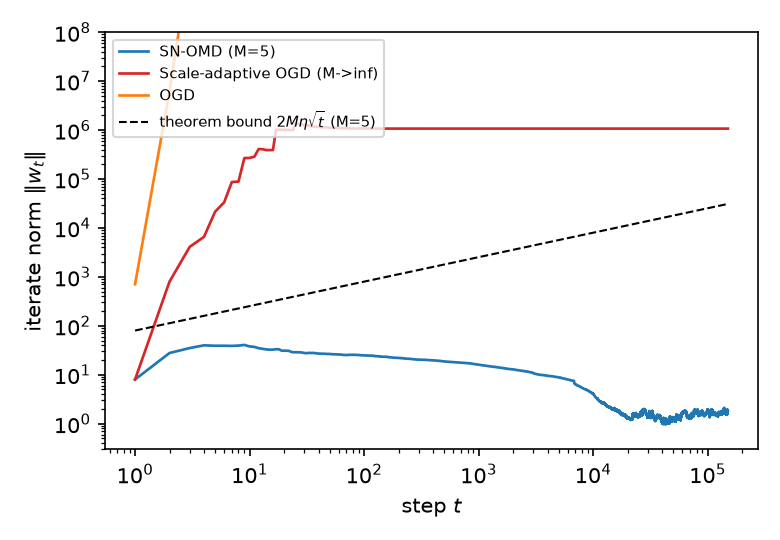
\includegraphics[width=0.6\linewidth]{fig8_iterate_norm.png}
\caption{\textbf{The bounded scale-free cap holds the iterate norm under the stability
envelope.} Iterate norm $\norm{w_t}$ (log--log) on $\mathrm{date}[0,120)$ at a shared rate
$\eta=8$. SN-OMD ($M=5$) stays below the theorem bound $2M\eta\sqrt t$ (dashed) at every
step; the uncapped endpoint ($M\!\to\!\infty$) and OGD blow through it (OGD exits the top).
This measures directly the $\norm{w_t}$ that \cref{thm:stability} bounds.}
\label{fig:iternorm}
\end{figure}

\subsection{Clipped moment and bias}
\begin{lemma}
\label{lem:clip}
For $v\in\R^d$, $M>0$, $p\in(1,2]$: $\norm{\clip(v,M)}^2\le M^{2-p}\norm v^p$ and
$\norm{v-\clip(v,M)}\le\norm v^p/M^{p-1}$.
\end{lemma}
\begin{proof}
If $\norm v\le M$: $\clip(v,M)=v$ and $\norm v^2=\norm v^p\norm v^{2-p}\le\norm v^p
M^{2-p}$, while $v-\clip(v,M)=0$. If $\norm v>M$: $\norm{\clip(v,M)}^2=M^2=M^pM^{2-p}
\le\norm v^pM^{2-p}$, and $\norm{v-\clip(v,M)}=\norm v-M\le\norm v=\norm v^p\norm
v^{1-p}<\norm v^pM^{1-p}$.
\end{proof}
\begin{lemma}[Moment and bias under \cref{ass:track}]
\label{lem:moment}
There is a constant $\kappa$ with $\E[\norm{\hat g_t}^2\mid\mathcal F_{t-1}]\le
M^{2-p}\kappa$, and the bias $b_t=\E[v_t-\hat g_t\mid\mathcal F_{t-1}]$ obeys
$\norm{b_t}\le\kappa/M^{p-1}$.
\end{lemma}
\begin{proof}
Take conditional expectations in \cref{lem:clip} with $v=v_t$ and use
$\E[\norm{\gt}^{p_t}\mid\mathcal F_{t-1}]\le\kappa_0\sigma_t^{p_t}$ and
$s_t\ge c_1\sigma_t$: $\E\norm{\hat g_t}^2\le M^{2-p}\E\norm{v_t}^p\le M^{2-p}
\kappa_0 c_1^{-p}$, and $\norm{b_t}\le\E\norm{v_t}^{p_t}/M^{p_t-1}\le\kappa_0 c_1^{-p_t}
/M^{p-1}$ (using $M\ge1$, $p_t\ge p$). Set $\kappa=\kappa_0 c_1^{-2}$, which dominates both
$\kappa_0 c_1^{-p}$ and $\kappa_0 c_1^{-p_t}$ since $c_1\le1$ and $p,p_t\le2$
(\cref{ass:track}).
\end{proof}
Because $M\ge1$ and $p_t\ge p$, all uses of $M^{2-p_t},M^{-(p_t-1)}$ above are bounded
by the worst-case $M^{2-p},M^{-(p-1)}$; the single-$p$ bounds are thus valid for
drifting $p_t$.

\subsection{High probability}
\begin{lemma}[Freedman step]
\label{lem:freedman}
Let $(X_t)$ be a martingale difference sequence with $|X_t|\le b$ and
$\sum_{t\le T}\E[X_t^2\mid\mathcal F_{t-1}]\le V$ almost surely. Then w.p.\ $\ge1-\delta$,
$\sum_{t\le T}X_t\le\sqrt{2V\log(1/\delta)}+\tfrac{2b}{3}\log(1/\delta)$. In particular,
for feedback $Z_t$ with $\norm{Z_t}\le B$ and $X_t=\ip{Z_t-\E[Z_t\mid\mathcal F_{t-1}]}
{w_t-u_t}$ ($u_t$ \emph{predictable}, i.e.\ $\mathcal F_{t-1}$-measurable, so $X_t$ is a
martingale difference; $\norm{w_t-u_t}\le D$), one may take $b=2BD$ and
$V=D^2\sum_t\E[\norm{Z_t}^2\mid\mathcal F_{t-1}]$.
\end{lemma}
\begin{proof}

$(X_t)$ is a martingale difference sequence ($\E[X_t\mid\mathcal F_{t-1}]=0$).
Freedman's inequality gives $\Pr(\sum_t X_t\ge\lambda)\le\exp(-\lambda^2/(2V+2b\lambda/3))$;
inverting the right-hand side to $\delta$ and using $\sqrt{x+y}\le\sqrt x+\sqrt y$ yields
the bound. For the instantiation, $|X_t|\le\norm{Z_t-\E[Z_t\mid\mathcal F_{t-1}]}\,
\norm{w_t-u_t}\le2BD$ and $\E[X_t^2\mid\mathcal F_{t-1}]\le D^2\E[\norm{Z_t}^2\mid
\mathcal F_{t-1}]$ since $\E\norm{Z-\E Z}^2\le\E\norm Z^2$.
\end{proof}

\subsection{Varying-step telescope}
\begin{lemma}
\label{lem:telescope}
SN-OMD is OGD with step $\eta_t=\eta/s_t$ on the clipped raw gradient. For any
comparator sequence $u_{1:T}$, writing $W_s=s_1+\sum_t(s_t-s_{t-1})_+$ and
$P_T^s=\sum_t s_t\norm{u_t-u_{t-1}}$,
\[
\sum_{t=1}^T s_t\bigl(\norm{w_t-u_t}^2-\norm{w_{t+1}-u_t}^2\bigr)\le D^2W_s+2D\,P_T^s.
\]
\end{lemma}
\begin{proof}
Write $s_0:=0$, so that $W_s=\sum_{t=1}^T(s_t-s_{t-1})_+$. Shifting the index in the
subtracted term, $\sum_{t=1}^T s_t\norm{w_{t+1}-u_t}^2=\sum_{t=2}^{T+1}s_{t-1}
\norm{w_t-u_{t-1}}^2$, hence
\[
\sum_{t=1}^T s_t\bigl(\norm{w_t-u_t}^2-\norm{w_{t+1}-u_t}^2\bigr)
=\sum_{t=1}^T\bigl(s_t\norm{w_t-u_t}^2-s_{t-1}\norm{w_t-u_{t-1}}^2\bigr)
 -s_T\norm{w_{T+1}-u_T}^2,
\]
and the final boundary term is nonpositive and dropped. Splitting each summand into a
comparator-move and a scale-change part,
\[
s_t\norm{w_t-u_t}^2-s_{t-1}\norm{w_t-u_{t-1}}^2
=s_t\bigl(\norm{w_t-u_t}^2-\norm{w_t-u_{t-1}}^2\bigr)+(s_t-s_{t-1})\norm{w_t-u_{t-1}}^2,
\]
which is at most $2D s_t\norm{u_t-u_{t-1}}+(s_t-s_{t-1})_+D^2$ by the reverse triangle
inequality and $\norm{\cdot}\le D$. Summing over $t$ gives $2D P_T^s+D^2 W_s$.
\end{proof}

\subsection{Dynamic regret (\texorpdfstring{\cref{thm:regret}}{Theorem 2})}

\paragraph{Roadmap and where each assumption enters.} The linearized regret splits into
three sums---(A) optimization, (B) martingale, (C) clipping bias---each closed by the
lemmas below. (A) uses the varying-step telescope (\cref{lem:telescope}) for the comparator/
scale-drift terms and the clipped second moment (\cref{lem:clip,lem:moment}) for the
curvature (whose random sum is concentrated by a second application of \cref{lem:freedman});
(B) uses the Freedman step (\cref{lem:freedman}); (C) uses the clipping-bias
bound (\cref{lem:moment}). The two assumptions enter in a few isolated places:
\cref{ass:moment} (finite $p$-th moment) only through \cref{lem:moment}, which converts
$\E\norm{\gt}^{p_t}\le\sigma_t^{p_t}$ into the conditional second-moment and bias bounds
of (A)--(C); \cref{ass:track}'s \emph{lower} bracket $s_t\ge c_1\sigma_t$ in the
curvature of (A)/(B) and the bias of (C); and its \emph{upper} bracket $s_t\le c_2\sigma_t$
in exactly one further place---the range constant $b_A$ of the curvature concentration in (A)
below (any predictable a.s.\ upper bound on $s_t$ would serve), never the exponent. So
over-estimating the scale is harmless to the \emph{rate}, costing only that Freedman range
constant. The dependency is
$\cref{lem:clip}\!\to\!\cref{lem:moment}\!\to\!\{\text{(A),(B),(C)}\}$, with
\cref{lem:telescope} feeding (A) and \cref{lem:freedman} feeding (B); the final display
balances (A)'s curvature against (C)'s bias through the choice of $\eta$ and $M$.

Write $d_t:=\clip(\gt,Ms_t)=s_t\hat g_t$ for the clipped \emph{raw} gradient, so that
SN-OMD is exactly OGD with adaptive step $\eta_t=\eta/s_t$ on $d_t$
(\cref{lem:telescope}). By convexity $R_T(u_{1:T})\le\sum_t\ip{\bar g_t}{w_t-u_t}$, and
we split the true subgradient as $\bar g_t=m_t'+\beta_t$, where
$m_t'=\E[d_t\mid\mathcal F_{t-1}]$ and $\beta_t=\bar g_t-m_t'=\E[(\gt-d_t)\mid
\mathcal F_{t-1}]$ is the (raw) clipping bias. Then
\begin{equation*}
\sum_t\ip{\bar g_t}{w_t-u_t}
=\underbrace{\sum_t\ip{d_t}{w_t-u_t}}_{\text{(A) optimization}}
+\underbrace{\sum_t\ip{m_t'-d_t}{w_t-u_t}}_{\text{(B) martingale}}
+\underbrace{\sum_t\ip{\beta_t}{w_t-u_t}}_{\text{(C) bias}}.
\end{equation*}
\emph{(A)} The OGD one-step inequality with step $\eta_t$, summed and combined with
\cref{lem:telescope}, gives
$\sum_t\ip{d_t}{w_t-u_t}\le\tfrac{1}{2\eta}(D^2W_s+2D P_T^s)+\tfrac{\eta}{2}
\sum_t\norm{d_t}^2/s_t$. Since $\norm{d_t}^2=\norm{\clip(\gt,Ms_t)}^2\le
(Ms_t)^{2-p}\norm{\gt}^p$ (\cref{lem:clip}) and $s_t\ge c_1\sigma_t$
(\cref{ass:track}), the curvature sum has conditional mean
$\le M^{2-p}\kappa'\sum_t\sigma_t=M^{2-p}\kappa'S_1$, with $S_1=\sum_t\sigma_t$ and
$\kappa'{:=}\kappa_0 c_1^{1-p}$ an absolute constant (the moment/lower-bracket constants of
\cref{ass:moment,lem:moment}). The curvature sum $\sum_t\norm{d_t}^2/s_t$ is itself random,
so its conditional-mean bound must be promoted to hold with high probability, not used
pathwise: apply \cref{lem:freedman} a second time to the predictable-variance sequence
$\xi_t:=\norm{d_t}^2/s_t-\E[\norm{d_t}^2/s_t\mid\mathcal F_{t-1}]$. The clip gives
$0\le\norm{d_t}^2/s_t\le M^2 s_t\le M^2 c_2\sup_t\sigma_t=:b_A$ (\cref{ass:track}), and
$\sum_t\E[\xi_t^2\mid\mathcal F_{t-1}]\le b_A\,M^{2-p}\kappa'S_1=:V_A$, so with probability
$\ge1-\delta$
\[
  \sum_t\norm{d_t}^2/s_t\;\le\;M^{2-p}\kappa'S_1
   +\sqrt{2V_A\log(1/\delta)}+\tfrac{2}{3}b_A\log(1/\delta).
\]
After the $\eta$-balance below, these deviations \emph{multiply} the leading term
$L=(D\sqrt{W_s}+\sqrt{D P_T^s})\sqrt{S_1}\,T^{(2-p)/(2p)}$ of \eqref{eq:mainbound}: the tuned
$\eta$ makes $\tfrac{\eta}{2}\cdot(\text{mean})=\Theta(L)$, so each deviation contributes
$\Theta(L)$ times its ratio to the conditional mean $M^{2-p}\kappa'S_1$. Writing
$\bar\sigma:=S_1/T$ for the mean scale, those ratios are
\[
\frac{\sqrt{2V_A\log(1/\delta)}}{M^{2-p}\kappa'S_1}
 =\Theta\!\Bigl(\sqrt{\tfrac{\sup_t\sigma_t}{\bar\sigma}\,\log\tfrac1\delta}\Bigr),
\qquad
\frac{\tfrac23 b_A\log(1/\delta)}{M^{2-p}\kappa'S_1}
 =\Theta\!\Bigl(\tfrac{\sup_t\sigma_t}{\bar\sigma}\,\log\tfrac1\delta\Bigr),
\]
both $O(1)$ in the horizon---no change to the $T^{1/p}$ exponent---but with constant the
\emph{peak-to-mean scale ratio} $\sup_t\sigma_t/\bar\sigma$, entering \emph{linearly} on the
range branch. Since $\sup_t\sigma_t/\bar\sigma\ge1$, that range branch \emph{dominates} the
square-root variance branch, so the curvature concentration multiplies $L$ by
$(\sup_t\sigma_t/\bar\sigma)\log(1/\delta)$---the leading-term multiplier reported in
\eqref{eq:mainbound}, not a $\sqrt{\log}$ factor. On a spiking scale this ratio is far from
$O(1)$; it is large precisely because of the volatility clustering this paper studies
(\cref{sec:experiments}), so the price of a high-probability curvature bound is itself a form
of the scale drift---a genuine constant cost, not a benign one. This is the step that makes
term~(A)---like (B)---a high-probability, not an in-expectation, bound.
\emph{(B)} The increments $\ip{m_t'-d_t}{w_t-u_t}$ form a martingale difference with
$\norm{d_t}\le Ms_t$ and $\E[\norm{d_t}^2\mid\mathcal F_{t-1}]\le M^{2-p}\kappa'
\sigma_t^2$; \cref{lem:freedman} bounds this sum by
$\tilde O(D M^{1-p/2}\sqrt{\sup_t\sigma_t\cdot S_1}\,)$, the same order as (A). This step
requires $u_t$ predictable (\cref{lem:freedman}), so the Freedman event is
comparator-specific; \cref{thm:regret} is accordingly a guarantee \emph{per fixed}
$u_{1:T}$, not one holding uniformly over all comparators (which would need a union or
chaining bound over comparator sequences, not pursued here).
\emph{(C)} $\norm{\beta_t}\le\E[\norm{\gt}^p\mid\mathcal F_{t-1}]/(Ms_t)^{p-1}\le
\kappa'\sigma_t/M^{p-1}$ (\cref{lem:moment}), so (C) $\le D\kappa'S_1/M^{p-1}$.
Choosing $\eta=\Theta\bigl(\sqrt{(D^2W_s+D P_T^s)/(M^{2-p}S_1)}\bigr)$ and
$M=\Theta(T^{1/p})$ balances the curvature term of (A) against the bias (C) and yields
\begin{equation*}
R_T(u_{1:T})=O\bigl(\sqrt{(D^2W_s+D P_T^s)\,M^{2-p}S_1}+D S_1/M^{p-1}\bigr),
\end{equation*}
which with $M=\Theta(T^{1/p})$ equals $(D\sqrt{W_s}+\sqrt{D P_T^s})\sqrt{S_1}\,
T^{(2-p)/(2p)}$ up to the bias term. Promoting the random sums (A) and (B) to high probability
multiplies this leading term by the curvature concentration's
$(\sup_t\sigma_t/\bar\sigma)\log(1/\delta)$ (the (A) range branch, dominating the
$\sqrt{\log(1/\delta)}$ variance branches) and adds the (B) Freedman range
$(\sup_t\sigma_t)D\,T^{1/p}\log(1/\delta)$, giving \eqref{eq:mainbound}. \emph{If} the scale
variation were bounded,
$W_s=O(1)$, and using $S_1\le T\sup_t\sigma_t$, this collapses to
$\tilde O((\sup_t\sigma_t)(D+\sqrt{D P_T})T^{1/p}\log(1/\delta))$---but $W_s$ is a data
quantity, and we \emph{measure} $W_s\sim T$ (\cref{sec:tracker}). So the $\sqrt{W_s}$
factor is a genuine $\sqrt T$ rate and this $T^{1/p}$ simplification holds only \emph{per
regime}; globally the bound is $T^{1/p+1/2}$ (at $p=2$, the vacuous $T$). The stationary
case ($\sigma_t\equiv\sigma$, $p=2$, no drift so $W_s=\sigma$) recovers
$\sigma(D+\sqrt{DP_T})\sqrt T$, the classical dynamic-OGD rate. \qed

\subsection{Reductions}
\emph{Unknown $p$:} $M=\Theta(T^{1/p})$ needs $p$; a doubling schedule over $M$, using
that the bound is unimodal in $\log M$ with a flat optimum, removes this at a
$\mathrm{polylog}(T)$ cost \citep{liu2026oco}. \emph{Unknown $\norm u$ / unbounded
domain:} \cref{thm:stability} gives bounded feedback $\norm{\hat g_t}\le M$, exactly
the input required by the parameter-free potential of \citet{zhangcutkosky2022};
substituting our $\hat g_t$ yields the unbounded-domain analogue with $D$ replaced by
$\norm u$. \emph{Unknown regime length:} \cref{lem:telescope} plus the interval version
of \cref{lem:freedman} give SN-OMD an interval-regret guarantee on every $[a,b]$; a
strongly-adaptive wrapper \citep{daniely2015,cutkosky2020} then recovers the dynamic
bound without knowing the regime structure, at a $\mathrm{polylog}$ overhead. A
per-regime transition cost $O(D\,N\,\mathrm{polylog}\,T^{1/p})$ is incurred while the
scale tracker re-concentrates after each of the $N$ regime changes; it is dominated
when regimes are macroscopic.

\subsection{Discharging \texorpdfstring{\cref{ass:track}}{the scale-tracking assumption}: a bracket guarantee}
\label{app:bracket}

\cref{ass:track} posits a predictable scale that brackets $\sigma_t$. We sketch why it is
not an oracle: under a mild model of the drift (piecewise-slow variation plus within-regime
mixing), the two-timescale envelope of \cref{sec:tracker} meets the essential lower bracket
off a small exceptional set, so the burden moves from ``an accurate scale estimate exists''
to ``the drift is piecewise slowly varying with a mixing scale,'' and the estimate is then
\emph{derived} from robust concentration. This is a sketch, not a theorem: the
window-median step needs a blocking argument (below), which we state as an assumption rather
than discharge.

\begin{figure}[t]
\centering
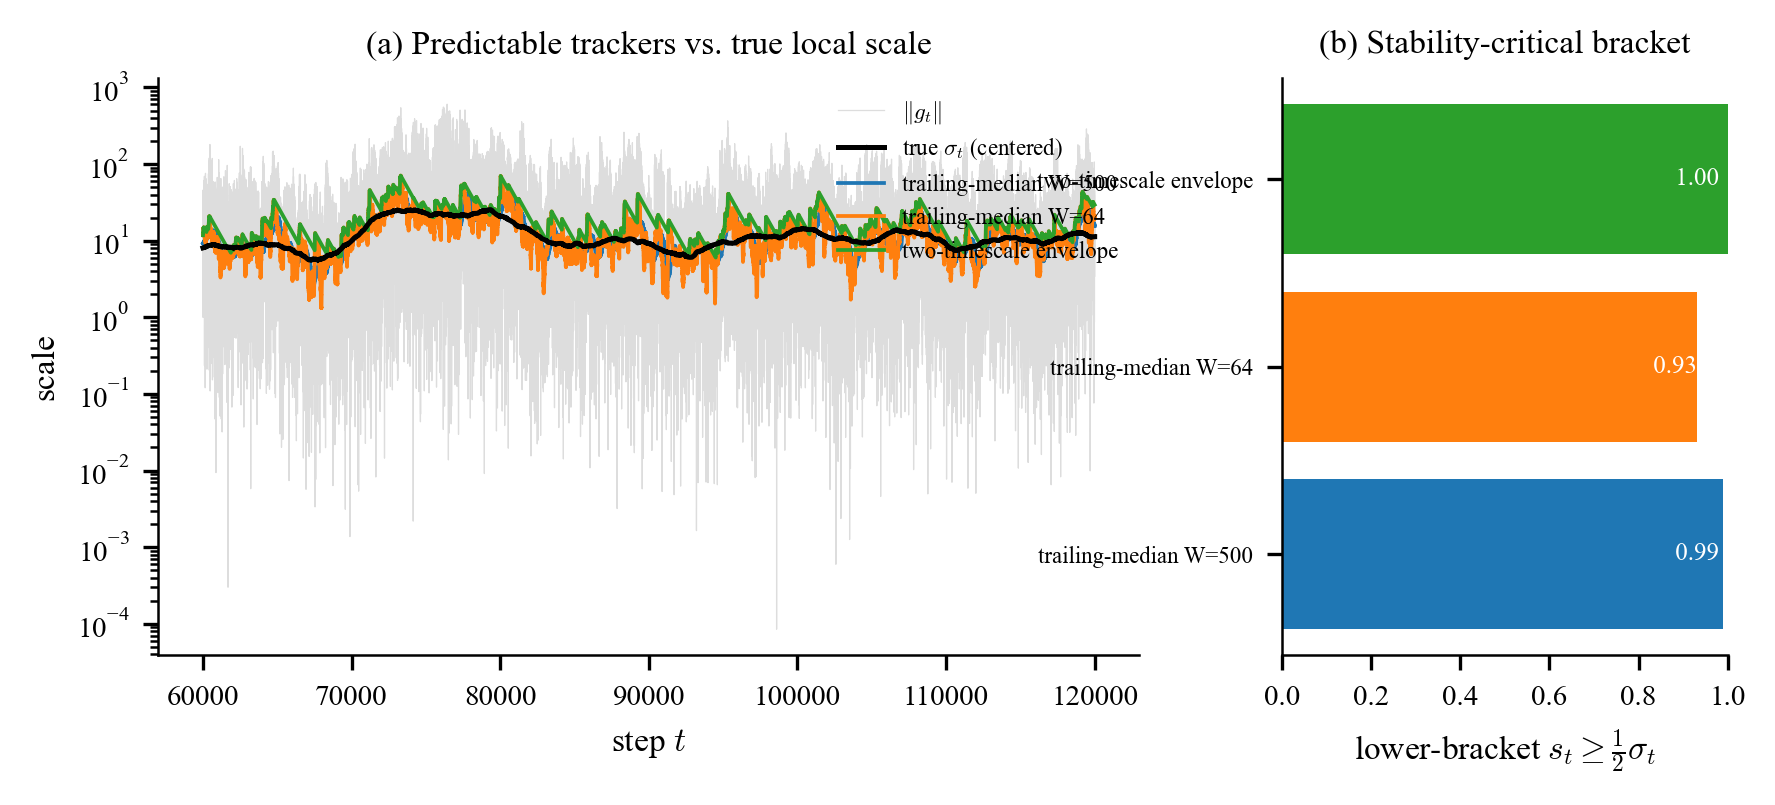
\includegraphics[width=\columnwidth]{fig4_tracker.png}
\caption{\textbf{Discharging \cref{ass:track}} (\cref{sec:tracker}). A two-timescale
``peak-hold'' tracker on the real gradient-scale process (a)~holds the lower bracket
$s_t\ge\tfrac12\sigma_t$ at every round while (b)~attaining the smallest upward variation
$W_s/V_\sigma^+$; a fast trailing median churns ($60\times$), a slow one lags and
violates the bracket.}
\label{fig:tracker}
\end{figure}

\begin{table}[t]
\caption{\textbf{Scale trackers on the real gradient-scale process} (\cref{sec:tracker}).
The two-timescale envelope holds the lower bracket at $100\%$ with the smallest upward
variation $W_s$. $V_\sigma^+$ is the true upward scale drift.}
\label{tab:tracker}
\centering
\begin{small}
\begin{tabular}{lccc}
\toprule
Tracker & Lower bracket & $W_s$ & $W_s/V_\sigma^+$ \\
\midrule
Trailing median, fast ($W{=}64$)   & $0.93$ & $38.6\mathrm{k}$ & $60\times$ \\
Trailing median, slow ($W{=}500$)  & $0.99$ & $5.0\mathrm{k}$  & $7.9\times$ \\
\textbf{Two-timescale envelope (ours)} & $\mathbf{1.00}$ & $\mathbf{4.2\mathrm{k}}$ & $\mathbf{6.6\times}$ \\
\bottomrule
\end{tabular}
\end{small}
\end{table}

\subsection{Synthetic streams: known tail and the cap sweep}
\label{sec:synthetic}\label{app:sweep}
On synthetic streams with a controlled tail (Student-$t$ index $p$; \cref{fig:synthetic}),
plain OGD's fitted cumulative-regret exponent rises $0.37\!\to\!0.70\!\to\!1.55$ as $p$
falls $2\!\to\!1.3$---super-linear (divergent) once the tail is heavy---reproducing the
real-data divergence with a \emph{known} tail index, so the tail is the mechanism, not a
learning-rate artifact. SN-OMD stays sublinear, with exponents \emph{below} $1/p$ (the
stochastic stationary instance is easier than the worst case, so this is consistent with,
not a tightening of, \cref{thm:regret}); against a drifting comparator its dynamic regret
grows with path length at exponent $\approx0.43$, consistent with the $\sqrt{D P_T}$ term.

\paragraph{The cap sweep (\cref{fig:msweep}).} Sweeping $M$ turns the cap into a
\emph{mechanism test}: normalization lightens but does not erase the tail
($\hat\alpha\!:2.4\to2.9$--$3.7$), so a finite cap should earn accuracy in proportion to the
\emph{residual} normalized heaviness. With an \emph{imposed} heavy normalized tail ($p{=}1.5$)
the finite-$M$ interior optimum is \emph{sharp}, beating the uncapped endpoint $\approx240\times$
(heavy-tail instability) and the normalized-GD ($M\!\to\!0$) endpoint $\approx10\times$
(magnitude-blind oscillation), both outside the seed-noise band. On Jane the same sweep, re-run
across the ten frozen windows (\texttt{research\_cap\_sweep\_jane.py}), has a \emph{broad,
shallow} interior optimum: a finite cap still beats full normalization ($M\!\to\!0$) by
${+}0.07$ (winsorized-EMA tracker, optimum $M{\approx}2$) to ${+}0.11$ (block tracker, optimum
$M{\approx}5$--$7$) and the uncapped endpoint diverges, but the mid-range caps are within seed
noise---matching Jane's \emph{milder} residual tail. So the earlier ``no accuracy on Jane''
reading was too strong: the cap buys accuracy on Jane too, modestly and broadly rather than in
the synthetic stream's sharp peak, and \emph{stability unconditionally}: uncapped scale-adaptive
OGD diverges at $\mathrm{lr}\ge2$ while SN-OMD does not.

\subsection{A second market (crypto), and an image-model boundary}
\label{app:secondmarket}
\paragraph{Crypto: the mechanism replicates on an independent market.} We repeat the whole
analysis on Binance BTC/USDT hourly bars ($76{,}888$ bars, 2017--2025, spanning the 2018 bear,
the 2020 COVID crash, the 2021 bull run, and the 2022 crash), predicting the next-hour log return
from causal features (lagged returns, rolling volatility, volume, intraday seasonality) with the
\emph{same} linear weighted-squared-loss task, gradient at the best fixed predictor, and
estimators (Hill $k{=}2000$; winsorized-EMA tracker, decay $0.99$) as on Jane
(\texttt{research\_crypto\_mechanism.py}). The mechanism replicates, and more sharply: the pooled
gradient tail is \emph{heavier} than Jane's ($\hat\alpha\approx1.81$ vs $2.4$; below $2$, i.e.\
infinite variance) and heavier than its own factors (residual $2.68$, feature $3.94$---the same
interaction effect); the causal scale tracker lightens it to $\hat\alpha\approx2.26$ ($+0.45$)
and a non-causal median to $2.40$; and---the decisive control---a marginal-preserving order
shuffle \emph{abolishes} the lightening (real $\Delta\hat\alpha={+}0.45$ vs shuffled
${-}0.01\!\pm\!.02$ over five seeds), so removability is again a property of \emph{serial
dependence}, not the marginal. The nonstationarity is stronger than Jane's: the daily gradient
scale drifts $22\times$ (Jane $6\times$) and the rolling $90$-day Hill $\hat\alpha$ is below $2$
on all $35$ windows. The honest difference from Jane is sharper, and we test it with the same
tool. A light-innovation surrogate---crypto's own volatility path and features fed \emph{Gaussian}
residual innovations, so \emph{zero} genuine tail by construction---run through the identical
pipeline normalizes causally to a \emph{light} $\hat\alpha\approx3.77$ (a failing tracker would
leave it heavy); a non-causal twin of the \emph{same} EMA lifts it only to $4.37$, so $3.77$ is a
genuine zero-tail floor, not a causal-estimation artifact. Yet the real normalized tail sits at
$2.26$, \emph{well below} that floor---and causality is not what limits it: the real stream's own
same-estimator causal-to-non-causal gap is only $+0.26$ ($2.26$ to $2.52$), squarely in the range
of Jane's ($+0.14$--$+0.38$ across thresholds and estimators; \cref{tab:residual}). Unlike
Jane---whose real $3.73$ sits \emph{at} its surrogate floor, i.e.\ no genuine tail beyond
estimation cost (\cref{tab:residual})---crypto's leftover is a \emph{genuine} heavy innovation
tail (residual $\hat\alpha\approx2.68$) that scale-tracking does not remove. This is the honest
scope of the second market: the drift-driven \emph{removability} replicates (the shuffle control),
but crypto also carries genuine innovation heaviness Jane lacks---exactly the regime where the cap
earns its keep, as the sharper stability dichotomy below confirms.

\paragraph{Crypto: the stability dichotomy replicates.} Hourly returns are near-unpredictable
(best-fixed-linear $R^2\approx0.002$), so no method has a meaningful accuracy edge---the
informative axis is divergence (\texttt{research\_crypto\_algorithms.py}). At a competitive rate
($\mathrm{lr}{=}2$) across ten disjoint windows, plain OGD diverges on $10/10$ (peak loss
${\sim}10^{127}$) and the \emph{uncapped} $M\!\to\!\infty$ endpoint on $3/10$, while every
\emph{bounded scale-free} method---SN-OMD ($M{=}5$) and its block variant, normalized-GD, the
fixed-$\tau$ clip, AdaGrad-Norm, and Cutkosky--Mehta---stays bounded ($0/10$): exactly the Jane
partition. Sweeping the rate on the turbulent 2022 window (\cref{fig:crypto}), both
scale-\emph{dependent} methods explode above $\mathrm{lr}\!\approx\!0.5$---OGD to ${\sim}10^{75}$
and the uncapped $M\!\to\!\infty$ endpoint to $5.0{\times}10^{17}$---while every bounded method
stays bounded to $\mathrm{lr}{=}8$; the cap is decisive, holding SN-OMD ($M{=}5$) at a peak loss
of $6.6$ there.

\begin{figure}[t]
\centering
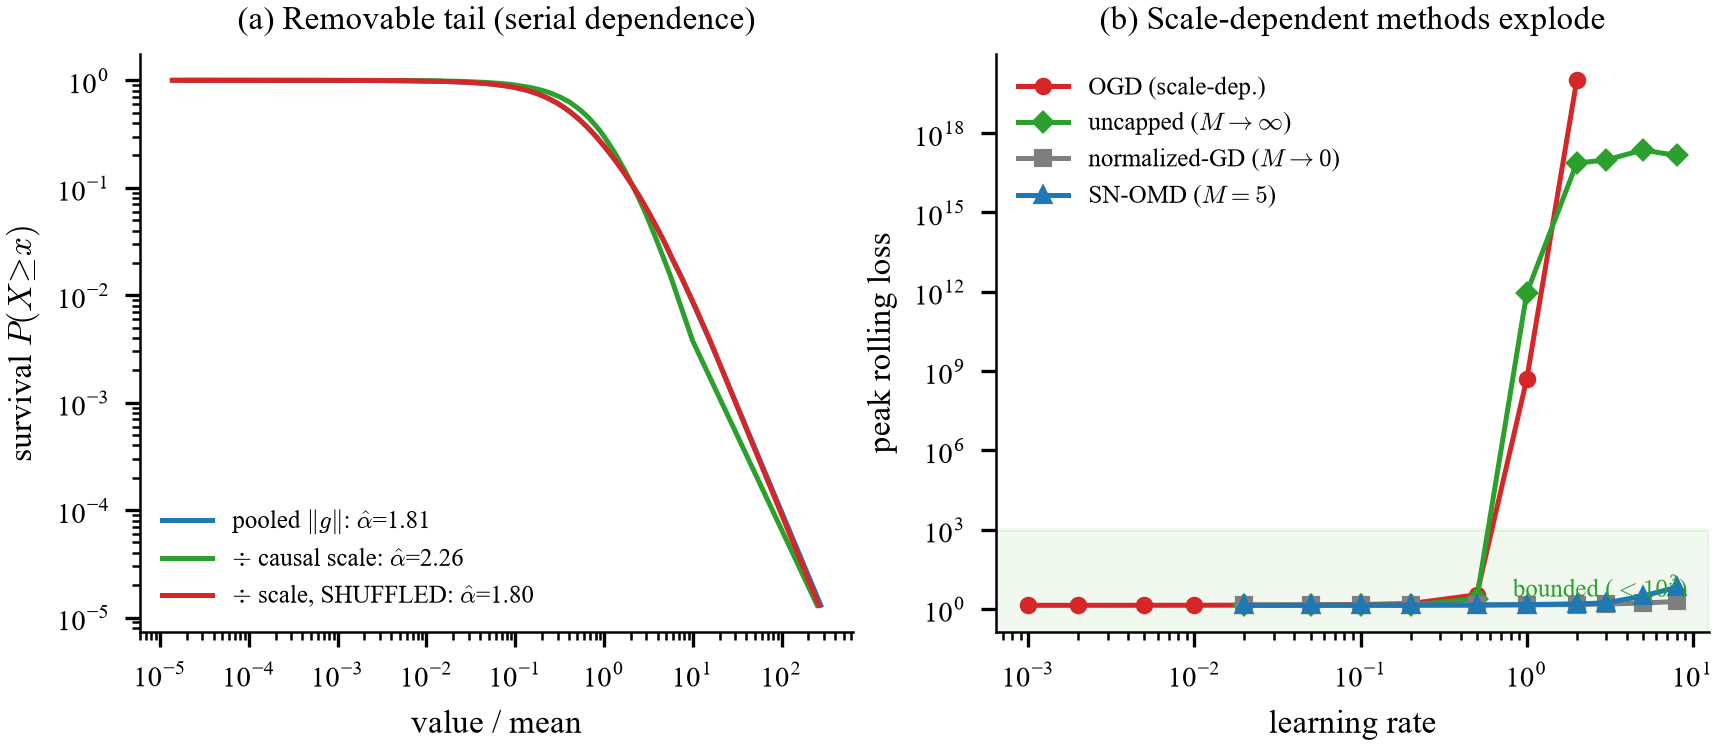
\includegraphics[width=0.9\columnwidth]{fig7_crypto.png}
\caption{\textbf{Second market (BTC/USDT 1h): mechanism and stability replicate}
(\cref{app:secondmarket}). (a)~Gradient-norm survival: the pooled tail ($\hat\alpha{=}1.81$) is lightened by the causal
scale tracker ($2.26$), and a marginal-preserving order shuffle \emph{abolishes} the lightening
($1.80$)---removability is serial dependence. (b) peak rolling loss vs.\ learning rate on the
turbulent 2022 window: the scale-dependent methods (OGD, uncapped $M\!\to\!\infty$) explode while
the bounded scale-free ones stay in the $<\!10^3$ band.}
\label{fig:crypto}
\end{figure}

\paragraph{Image models: a boundary, not a replication.} On the per-step gradient norm of a small
CNN on MNIST ($2{,}814$ steps) the pooled tail is heavy ($\hat\alpha\approx2.6$) and normalizing
lightens it, but this is \emph{schedule-driven}: within a constant-learning-rate window the tail
is already light ($\hat\alpha\approx6$--$9$), so the heaviness is scale decay, not within-phase
drift. This is a genuine boundary---training gradients need not carry the within-regime effect,
which we establish on the two \emph{market} streams.

\begin{figure}[t]
\centering
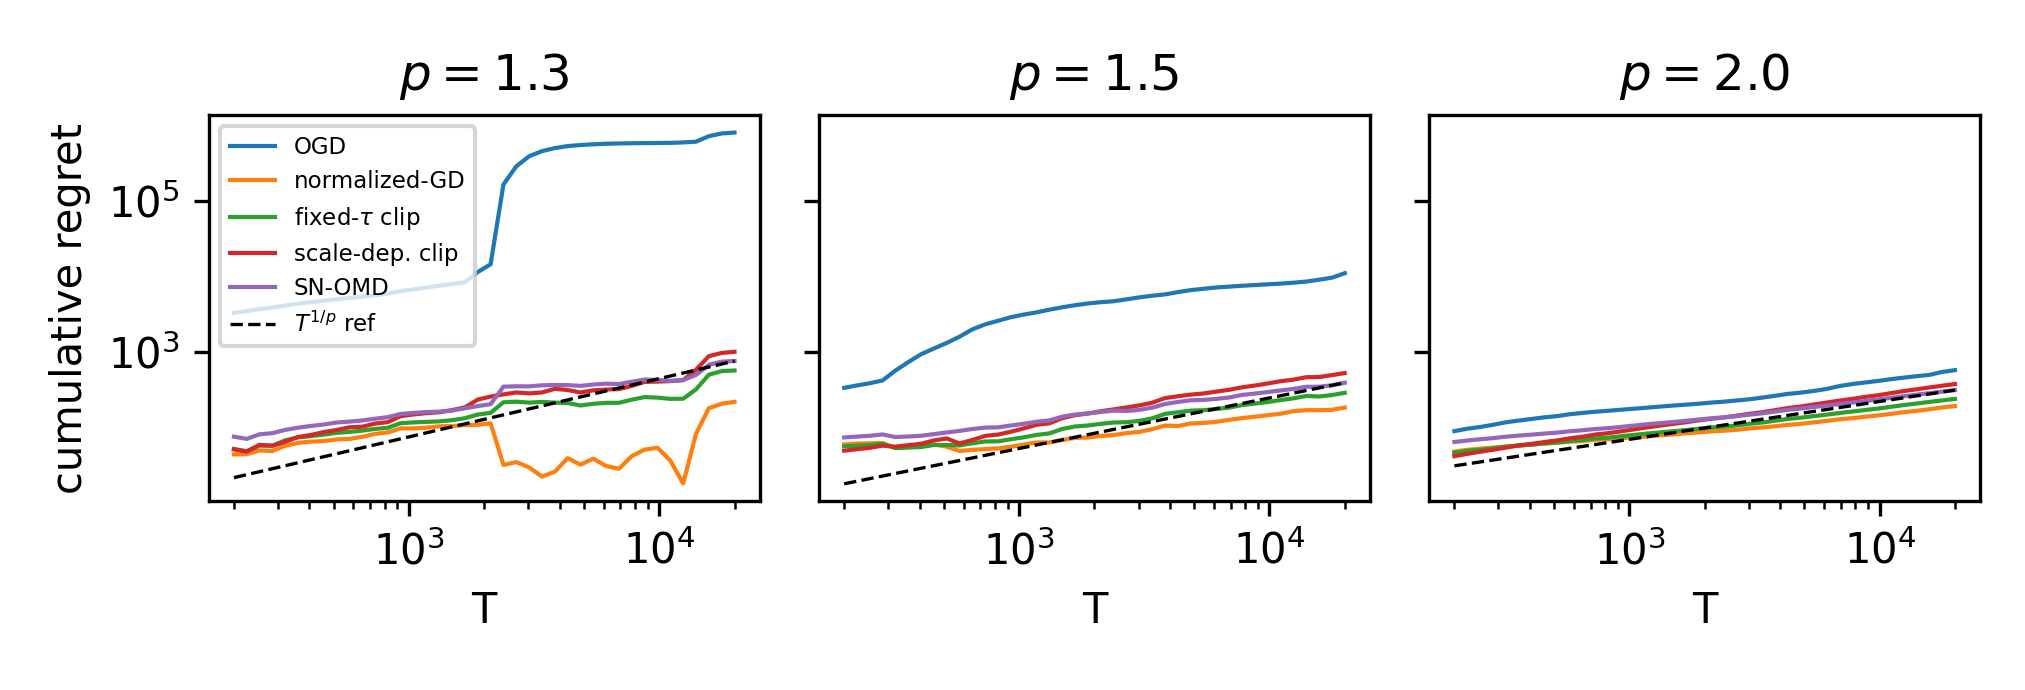
\includegraphics[width=\columnwidth]{fig5_synthetic.png}
\caption{\textbf{Known-tail synthetic} (\cref{sec:synthetic}). Cumulative regret vs.\ $T$
at $p\in\{1.3,1.5,2.0\}$: OGD's exponent climbs past $1$ (divergent) as the tail heavies,
while SN-OMD stays sublinear and below the $T^{1/p}$ reference (dashed).}
\label{fig:synthetic}
\end{figure}

\begin{figure}[t]
\centering
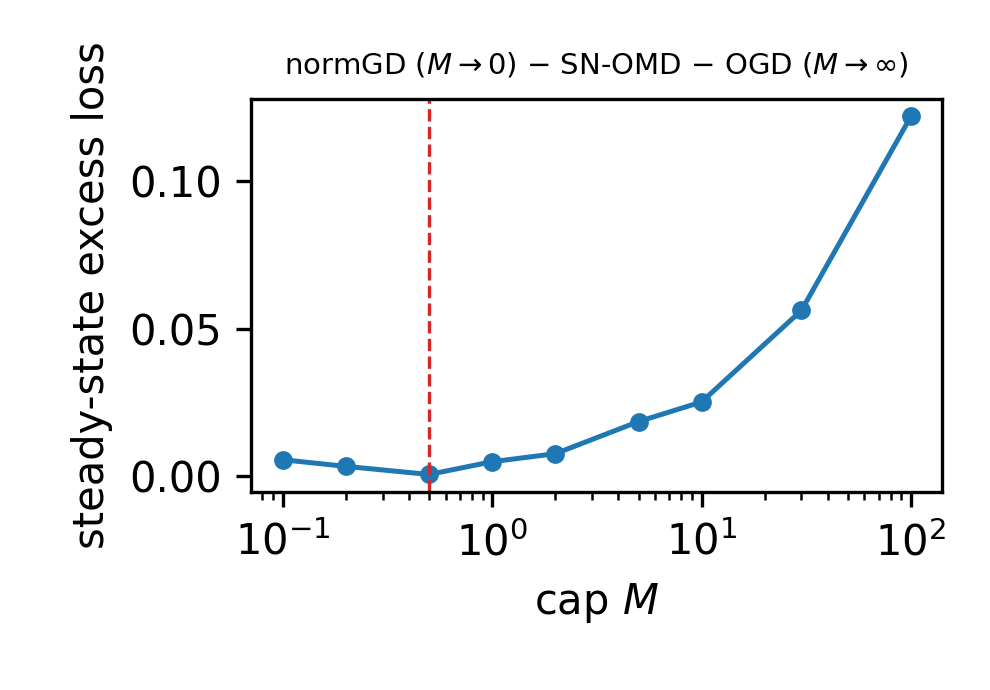
\includegraphics[width=0.72\columnwidth]{fig6_msweep.png}
\caption{\textbf{The cap has an interior optimum} (synthetic, $p=1.5$; \cref{sec:msweep}).
Steady-state excess loss vs.\ $M$, each cap at its own tuned step: the finite-$M$ optimum
beats both the normalized-GD end ($M\to0$) and the uncapped scale-adaptive-OGD end
($M\to\infty$).}
\label{fig:msweep}
\end{figure}

\begin{table}[t]
\caption{\textbf{The scale drift is a genuine rate, but its constant is controllable}
(\cref{sec:tracker}). Upward variation $W_s$ vs.\ the tracker's update block length $B$ (predictable robust
median per block) on the $200{,}000$-round gradient-scale process. Restricting the
$W_s\sim T^{\beta}$ fit to horizons with $\gtrsim\!50$ blocks gives $\beta\approx1.0$--$1.25$
where reliably measurable ($B{=}100,10^3$), with no monotone trend; the naive full-range
fit's decline (to $0.17$ at large $B$) is a finite-horizon artifact---$B{=}10^4$ has only
$\sim\!20$ blocks and no $\ge\!50$-block horizon. What $B$ controls is the constant,
shrinking $W_s$ by $\sim\!5$ orders of magnitude while roughly holding the lower bracket.
Escaping the resulting $\sqrt T$ drift factor needs a switching bound in the regime count,
left open.}
\label{tab:beta}
\centering
\begin{small}
\begin{tabular}{lccccc}
\toprule
block $B$              & $1$ & $100$ & $10^3$ & $3{\cdot}10^3$ & $10^4$ \\
\midrule
$W_s$ (full record)   & $1.8\mathrm{M}$ & $3216$ & $319$ & $108$ & $29$ \\
$\beta$ ($\ge\!50$ blk) & --- & $1.03$ & $1.25$ & $0.73$ & n/a \\
lower bracket         & $0.72$ & $0.97$ & $0.97$ & $0.92$ & $0.93$ \\
\bottomrule
\end{tabular}
\end{small}
\end{table}

\paragraph{Drift model.} Partition $[T]$ into $N$ regimes by change points
$t_0<\dots<t_N$. \emph{Slow within-regime drift:} inside a regime the scale varies
slowly, $\sigma_t/\sigma_{t-1}\in[1-\gamma,1+\gamma]$ with $\gamma W\le c_0$ for the
window $W$. \emph{Arbitrary jumps:} at the $N$ change points $\sigma_t$ may jump by any
factor. This is the piecewise-slowly-varying picture the measured gradient scale fits
($\sim\!30\%$ within-day drift, occasional $3\times$ overnight jumps; \cref{sec:experiments}).

\paragraph{Tracker.} The envelope $s_t=\max\{c\,\widehat m_t,\,(1-\rho)s_{t-1}\}$, where
$\widehat m_t=\mathrm{median}(\norm{g_{t-W}},\dots,\norm{g_{t-1}})$ is the predictable
short-window median and $\rho\asymp1/L$ with $L=\min_r L_r$.

\begin{proposition}[Bracket guarantee, informal]
\label{prop:tracker}
Under \cref{ass:moment}, the drift model above, and $\beta$-mixing of the within-regime
$\norm{\gt}$ process (so a blocking argument yields window-median concentration---the iid
order-statistic rate is otherwise only heuristic under the serial dependence documented in
\cref{sec:experiments}), for a large enough constant $c$, with probability $\ge1-\delta$:
\emph{(i, lower bracket)} $s_t\ge c_1\sigma_t$ for every $t$ outside at most $O(W)$
rounds after each jump---an exceptional set of size $O(NW)$; and
\emph{(ii, bounded variation)} $W_s=O(\sup_t\sigma_t+\rho\sum_t\sigma_t)=O(V_\sigma^+)$.
Consequently \cref{thm:regret} holds with one added term $O(D\,N\,W\,\sup_t\sigma_t)$,
dominated whenever $NW\ll T^{1/p}$ (macroscopic regimes).
\end{proposition}

\medskip\noindent\textit{Proof sketch (heuristic; the window-concentration step is the
$\beta$-mixing assumption, not a discharged bound).}
\emph{Window concentration.} On a window lying inside one regime, the population median
of $\norm{\gt}$ is a constant multiple of $\sigma_t$---a regular-variation/scale-family
assumption on the conditional law, \emph{beyond} the moment bound of \cref{ass:moment}. Under the
within-regime $\beta$-mixing assumption a blocking argument gives empirical-median
concentration around it---split the window into $\asymp W/\ell$ near-independent blocks of
length $\ell\gtrsim$ the mixing time; the iid order-statistic bound is the $\ell{=}1$
special case and is only heuristic under the serial dependence this paper documents. The
slow drift shifts the constants by $O(\gamma W)=O(1)$. Hence
$\widehat m_t\in[a\sigma_t,b\sigma_t]$ w.h.p., and $c\ge c_1/a$ gives
$c\,\widehat m_t\ge c_1\sigma_t$, so the $\max$ meets the lower bracket whenever the
window lies in one regime.
\emph{Jumps.} After an upward jump the window still holds pre-jump norms for $\le W$
rounds; during that lapse the median term may under-estimate, giving the $O(NW)$
exceptional set. A downward jump only makes $s_t$ conservatively high (the release lets
it fall at rate $\rho$), never violating the lower bracket.
\emph{Variation.} Upward moves of $s_t$ come only from $c\,\widehat m_t$ rising; between
jumps these telescope to $\sup_t s_t$, and the geometric release contributes the churn
$\rho\sum_t s_t$, so $W_s\le\sup_t s_t+\rho\sum_t s_t$, which is $O(V_\sigma^+)$ for
$\rho\asymp1/L$ (\cref{rmk:tracker}).
\emph{Exceptional rounds.} On the $O(NW)$ lapse rounds the update is still bounded
($\norm{\hat g_t}\le M$, \cref{thm:stability}) but the clipping bias (C) is uncontrolled;
charging it trivially at $O(D\sup_t\sigma_t)$ per round gives the added
$O(D\,N\,W\,\sup_t\sigma_t)$.\medskip

The blocking argument is not free: each block must span several mixing times, so the window
$W$ needed for concentration inflates with the mixing coefficient, and with it the $O(NW)$
exceptional set. The proposition therefore says something only for regimes long enough that
$NW\ll T^{1/p}$ \emph{survives} this inflation; for short or rapidly-mixing regimes the lapse
term is no longer dominated, and the guarantee degrades to the empirical discharge of
\cref{sec:tracker}. The residual---the post-jump lapse---is an additive term already of the form isolated in
the Reductions above, and making $\rho$ adaptive to an unknown $L$ is exactly the
strongly-adaptive wrapper of that subsection.

\subsection{Trackers: guarantee versus accuracy}
\label{app:tracker}

The regret analysis discharges \cref{ass:track} with the two-timescale ``peak-hold''
envelope of \cref{sec:tracker}, whereas the per-row \emph{accuracy}-optimal configuration is
the block median and the cheap reactive default is a winsorized exponential moving average
(EMA). Because the analyzed object and the reported object thus differ, we state precisely
what does and does not depend on the choice of tracker.

\paragraph{Stability is tracker-independent.} \cref{thm:stability} uses only
$\norm{\hat g_t}\le M$, which the cap enforces for \emph{any} predictable $s_t>0$.
Non-divergence therefore holds verbatim for the EMA, for the envelope, and for any
other tracker; the gap discussed here is never about stability, only about the leading
regret constant.

\paragraph{Only the regret constant depends on the tracker.} For any predictable $s_t$
meeting the essential lower bracket $s_t\ge c_1\sigma_t$, the rate is $T^{1/p}$
(\cref{thm:regret}); trackers differ only through the leading factor $\sqrt{W_s}$. The
envelope is the tracker for which we can \emph{prove} both the lower bracket and
$W_s=O(V_\sigma^+)$ (\cref{prop:tracker})---reacting up
on a short robust median and releasing down only geometrically keeps every upward move a
genuine rise (\cref{tab:tracker}: $100\%$ lower bracket, $W_s=6.6\,V_\sigma^+$). A fast,
\emph{unwinsorized} EMA can in principle churn on heavy-tailed $\norm{\gt}$ spikes
(\cref{tab:tracker}: $W_s=60\,V_\sigma^+$); winsorizing the EMA at $k\cdot\mathrm{median}$
caps each upward step and is what keeps the deployed default's $W_s$ finite in practice,
though we do not give it a closed-form bound.

\paragraph{Which tracker to deploy: a three-way gap, widest at the best point.} There are
now three trackers in play and the accuracy/guarantee trade-off has three corners.
\emph{(1) The envelope} $s_t=\max\{c\,\hat m_t,(1-\rho)s_{t-1}\}$ is the only one with a
\emph{proven} bound: \cref{prop:tracker} gives it both the lower bracket and
$W_s=O(V_\sigma^+)$. \emph{(2) The winsorized EMA} (deployed default) has no closed-form
$W_s$ bound---\cref{prop:tracker} does not cover it, as its functional form is not the
envelope's---only the empirical $W_s=60\,V_\sigma^+$ of \cref{tab:tracker}. \emph{(3) The
block median} ($B{=}10^4\approx$ one day) is among the most accurate \emph{per-row} on our
stream---tied with the normalize-and-clip baseline (\cref{tab:replication}), while per-step
the fixed-$\tau$ clip edges it on window~1 ($0.382$ vs.\ $0.351$; \cref{tab:jane})---yet
the least analyzed: \cref{prop:tracker} does not cover it either, and we prove nothing about its
$W_s$. So a best-performing tracker is again one with no guarantee; the gap between what we
can \emph{prove} (envelope) and what we would \emph{deploy} (EMA, or block) is if anything
wider than before. The ten-window replication (\cref{tab:replication}) makes this concrete:
holding hyperparameters frozen from window~1 and tuning each row's cap alongside its rate, the
block-median tracker lifts SN-OMD's per-row mean from $0.24$ to the co-leading $0.28$ while
\emph{widening} its across-window standard deviation ($0.05\!\to\!0.09$); neither row is
negative on any window. The across-window variability therefore tracks the cap setting rather
than the tracker, and the deploy question is sharpened rather than settled: the tracker that is
most accurate is exactly the one we cannot yet bound. This also resolves a single-window
observation: SN-OMD's per-row error bar in \cref{tab:jane} runs about twice normalized-GD's
($\pm.079$ vs.\ $\pm.037$, and no wider per-step), which the replication does \emph{not} trace
to the EMA tracker---once the cap is tuned alongside the rate the EMA is the \emph{tighter} of
the two SN-OMD rows across windows.

The accuracy gaps are easy to over-read, so we test them across regimes: the ten frozen
windows (\cref{tab:replication}) are the instrument that varies the hypothesized variable, so
we pair the block median against the EMA default and each baseline \emph{by window} and
bootstrap the paired difference over the ten windows
(\texttt{research\_tracker\_bootstrap.py}). Resampling at the \emph{window} granularity
absorbs the within-window serial dependence (volatility clustering); the only residual
assumption is that the ten paired differences are exchangeable across windows, which the
pairing de-risks by cancelling any regime effect common to both methods. Per-row the block
tracker beats every method
\emph{except one}, with a paired $95\%$ CI clear of zero and $10/10$ window wins---the EMA
default by $+0.15$ ($[+0.10,+0.20]$), normalized-GD by $+0.11$ ($[+0.08,+0.15]$), the
fixed-$\tau$ clip by $+0.085$, AdaGrad-Norm by $+0.093$---but only \emph{ties} the
normalize-and-clip Cutkosky--Mehta baseline ($+0.004$, CI $[-0.014,+0.023]$, $6/10$), which
co-leads. The paired instrument \emph{supersedes} the single-window block-bootstrap gap of
$+0.10$ (CI $[-0.04,+0.23]$) we reported in earlier drafts: that instrument \emph{fixes} the
regime, exactly the variable the effect lives in. The result is not a tracker-\emph{selection}
artifact either: dropping window~1---on which the block median was chosen---leaves the
significant gaps intact (EMA $+0.15$, $[+0.10,+0.21]$, $9/9$; normalized-GD $+0.10$, $9/9$) and
the CM tie unchanged ($+0.000$, $[-0.018,+0.018]$, $5/9$). The picture is
\emph{protocol-specific}: per-step the block tracker still does \emph{not} lead---it is
statistically tied with the fixed-$\tau$ clip ($-0.000$), AdaGrad-Norm ($+0.01$), and the EMA
default ($+0.07$)---but it no longer trails normalized-GD. That method's window-1-optimal
per-step rate overfits (\cref{app:grid}) and collapses across regimes, so block now \emph{beats}
it ($+0.11$, $[+0.05,+0.17]$, $8/10$), as it does the likewise-collapsed CM---which per-step
\emph{is} normalized-GD (clipping only rescales $\gt$, so at its no-momentum optimum $\beta{=}0$
the two are bit-identical, $0.09\!\pm\!.21$; \texttt{research\_cm\_normgd\_equiv.py}). Per-row,
CM's tie with the block tracker is almost all momentum: at $\beta{=}0$ it again reduces to
normalized-GD ($0.18\!\pm\!.01$), and of the $+0.10$ lift to $0.29$ the $\beta{=}0.5$ momentum
supplies ${+}0.09$ and the clip only ${+}0.01$ (removing it, $\tau\!\to\!\infty$, costs
${<}0.03$ on any window; \texttt{research\_cap\_sweep\_jane.py}). What the block tracker matches
with a \emph{predictable} scale, CM needs momentum to reach. Where block ties
the clip per-step, the mechanism is substitution: per-step batching averages the $\sim\!9$
correlated symbols in each $(\text{date},\text{time})$ group, and that averaging is itself the
variance reduction the smooth block scale supplies per-row, so the two do not compound---when
the protocol already smooths the update, a smoother tracker adds nothing.

\paragraph{Multiple comparisons.} The CIs above are uncorrected across the $14$ paired tests in
this subsection (seven baselines $\times$ two protocols; the drop-window-1 set re-analyses the
same comparisons rather than adding new ones). A Bonferroni correction at
$\alpha/14$ ($t_9$ critical value $3.91$ instead of $2.26$) changes two verdicts, both
\emph{per-step} and both already marginal: the gap over the uncapped scale-adaptive endpoint,
$+0.106$ with uncorrected CI $[+0.005,+0.208]$, becomes inconclusive ($[-0.069,+0.281]$), and so
does the gap over the EMA default, $+0.079$ ($[+0.004,+0.154]$ becoming $[-0.051,+0.208]$).
Neither is load-bearing: the tracker claim we make is the \emph{per-row} one. Every gap the paper's claims rest on
survives---per-row over the EMA default $+0.151$ ($[+0.065,+0.238]$), normalized-GD $+0.113$
($[+0.056,+0.170]$), the fixed-$\tau$ clip $+0.085$, AdaGrad-Norm $+0.093$, OGD $+0.290$, and
per-step over normalized-GD/CM $+0.107$ (marginally, $[+0.001,+0.213]$)---and every tie stays a
tie, the Cutkosky--Mehta co-lead ($+0.004$, $[-0.028,+0.036]$ corrected) included. We therefore
report uncorrected intervals and flag the two borderline results as suggestive.

\paragraph{Which tracker we report, and why.} We therefore report the block median as a
per-row \emph{co-optimal} tracker---it \emph{ties} the normalize-and-clip baseline at the top of
the ten-window ranking ($+0.004$, n.s.) and significantly beats the EMA default and the
remaining bounded baselines ($+0.08$ to $+0.15$, $10/10$)---while
being explicit that it is the plug-in with \emph{no} proven $W_s$ bound (\cref{prop:tracker}
covers only the envelope). SN-OMD's contribution is the normalize-and-cap update, stable for
\emph{any} predictable $s_t$ (\cref{thm:stability}); the tracker is a documented choice with a
measured trade-off---the block median when per-row accuracy is the goal, the envelope when the
$W_s$ guarantee is, the winsorized EMA as a cheap reactive default between them. We report
the block median because ten frozen windows put it at the top of the per-row ranking (tied),
not because it is the most analyzable---deploying the corner with no $W_s$ bound is a deliberate
choice, and we state it as one. Past the tuned range every tracker
\emph{degrades in loss} without diverging (\cref{thm:stability})---at $\mathrm{lr}{=}10$ the
peak rolling loss reaches $\approx30$ (block) or $\approx230$ (EMA) while the $O(\sqrt t)$
iterate bound holds---the block tracker most gracefully.

This may look in tension with \cref{sec:tracker}/\cref{fig:main}, where long windows are
penalized for lagging regime onsets. The tension is only apparent, and it is exactly the
distinction between the two uses of the scale. When the scale is a \emph{divisor}
($\hat{g}_t=\gt/s_t$), a lagging $s_t$ merely mis-normalizes the step magnitude---the divisor
cancels first-order and a slightly stale scale costs little, so a slow block median is
tolerable and even helpful (it is smoother and higher-bracket). We measured this rather than
asserting it: sweeping the tracker's block timescale over $B\in\{50,\dots,20{,}000\}$ (a
$400\times$ window range) moves the divisor's best-tuned weighted $R^2$ only within
$[0.363,0.386]$ (spread $0.022$), if anything \emph{rising} with the window---so a longer,
laggier scale does not hurt the normalizer. When the scale is instead a \emph{threshold}
(clipping $\norm{\gt}$ at $s_t$), the same sweep says something \emph{sharper} than ``long
windows hurt thresholding.'' The threshold use never leaves $R^2\approx0.003$ at \emph{any}
window: clipping $\norm{\gt}$ at a tracked scale is scale-\emph{dependent} OGD, stable only at
a tiny step ($\mathrm{lr}\approx3\times10^{-4}$), so it is unusable no matter how the scale is
tracked. Window choice is therefore moot on the threshold side---there is no usable operating
point to tune toward---while the divisor is usable and window-insensitive across the whole
$400\times$ range. This is the paper's central fragility finding (\cref{sec:experiments})
arriving from the tracker-design direction: normalization decouples the step from the scale and
thresholding does not, so the very lag that would wreck a threshold (it clips hardest exactly
when the scale jumps up, discarding the informative post-onset gradients---the
\cref{sec:tracker} clip-rate/dynamic-range tension) merely re-normalizes a divisor. The
one-day block tracker is a normalizer, so no contradiction arises.

\paragraph{Closing the gap.} Either run the envelope in deployment, accepting the small
accuracy cost, or prove a $W_s$ bound for the winsorized EMA under a heavy-tailed scale
process: the winsorization already supplies the per-step cap the envelope gets from its
median, so what remains is to control the geometric-decay churn term $\rho\sum_t s_t$,
exactly as in \cref{rmk:tracker}, with $\rho$ the EMA rate. The
one residual modeling assumption---$\rho$ matched to an unknown regime length---is
removed by the strongly-adaptive wrapper of the preceding subsection.

\subsection{Grid adequacy: window-1 optima are interior}
\label{app:grid}

\cref{tab:replication,tab:jane} tune each method's learning rate (and any second
hyperparameter) on window~1 and freeze it. A tuning grid whose optimum lies on a boundary can
silently truncate a method's performance---the failure that produced a misconfigured
Cutkosky--Mehta cell in an earlier draft, whose momentum grid $\beta\in\{0.9,0.99\}$ missed the
optimum at $\beta\!\to\!0$. We therefore checked every method:
\texttt{research\_grid\_adequacy.py} sweeps each method's full window-1 grid and reports whether
every tuned axis's optimum is strictly interior. It was not, at first---the scale-free family's
learning-rate optima sat at the old ceiling $\mathrm{lr}{=}2$. Widening the ceiling to $8$
(\texttt{research\_lr\_widen.py} confirms every curve peaks by $\mathrm{lr}{=}3$--$5$ and
declines past it) makes every accuracy-relevant optimum interior (\cref{tab:grid}).

This matters because it changed the reported numbers, against our interest. Three
window-1-optimal rates rose (normalized-GD $2\!\to\!3$ per-row and $2\!\to\!5$ per-step, block
$2\!\to\!3$ per-row), and---because a rate tuned to maximize \emph{one} window overfits it---%
normalized-GD's per-step number then \emph{fell} across the other nine, from $0.29$ (at the
truncated $\mathrm{lr}{=}2$) to $0.09\!\pm\!0.21$ (at the true optimum $\mathrm{lr}{=}5$). The
old, narrower grid was implicitly regularizing; the grid-adequate ranking is the one in
\cref{tab:replication}, where per-row the block-median SN-OMD ties the normalize-and-clip
baseline and per-step no member leads. This is the paper's regime-dependence thesis turned on
its own tuning: a rate optimal on the tuning window need not transfer. What does \emph{not}
move is the stability partition---every finite-cap method stays bounded ($0/10$) at its widened
optimum, and no higher frozen rate introduces a divergence---so raising the ceiling costs the
accuracy \emph{rankings} but not the stability claim the paper turns on.

\paragraph{The cap: where it is tuned, and where it is not.} \cref{tab:jane},
\cref{fig:main} and the cap sweeps fix $M{=}5$ a priori. \cref{tab:replication} does
\emph{not}: there both SN-OMD rows are tuned over $(\mathrm{lr},M)$ on window~1, so that SN-OMD
and the fixed-$\tau$ clip receive the same two-parameter budget---$70$ configurations each, with
$M$ swept over $[0.5,100]$ against $\tau$ over $[2,300]$
(\texttt{research\_c12\_matched\_table.py}, \texttt{research\_c12b\_blockmed.py}). An earlier
draft pinned $M{=}5$ there while sweeping $\tau$, which is the tuning-budget asymmetry this
corrects. Three things follow. \emph{(i)~The a-priori $M{=}5$ was not conservative for the block
tracker.} On window~1 its per-row $R^2$ keeps rising past $M{=}5$ (to $0.42$ at $M{=}10$), which
would read as $M{=}5$ being timid---but that is a window-1 overfit of exactly the kind above:
across the ten frozen windows the cap optimum is a \emph{broad plateau} at $M{=}5$--$7$ ($0.29$)
with $M{=}10$ falling back to $0.28$ (\texttt{research\_cap\_sweep\_jane.py}), and the
matched-budget run---which selects $M{=}10$ from window~1 alone---indeed lands at $0.28$ across
the ten, reproducing that sweep to $0.002$. \emph{(ii)~For the winsorized-EMA tracker the pinned
cap \emph{was} costing accuracy}: tuning it lifts the per-row mean from $0.14$ to $0.24$ and
narrows the across-window spread from $\pm.11$ to $\pm.05$, so the variability an earlier draft
attributed to that tracker belonged to the pinned cap. \emph{(iii)~The per-step selection is the
table's one boundary case}: it pins at both the rate ceiling ($\mathrm{lr}{=}8$) and the cap
floor ($M{=}0.5$), i.e.\ it collapses \emph{toward} the $M\!\to\!0$ normalized-GD endpoint. We
record this rather than defend it. It is the same per-step preference for a small cap that the
window-1 sweep found on the narrower range $[2,20]$ (footnote to \cref{tab:grid}), and it is a
further reason to read the per-step column as separating no member of the bounded family. That
same ten-window sweep re-derives the cap's mechanism test on Jane (\cref{app:sweep}).

\paragraph{The negative control is not a grid artifact.} The stationary control of
\cref{sec:experiments} tunes both learners over their own rate grids
(\texttt{research\_review3\_checks.py}), and tuned SN-OMD's optimum initially sat at that grid's
floor $\eta{=}0.05$, leaving open that a smaller rate rescues it. Widening the grid down to
$\eta{=}0.01$ does not: the optimum stays at $\eta^\star{=}0.05$---now strictly interior---with
steady excess loss $6.4\!\times\!10^{-4}$, against tuned OGD's $5.5\!\times\!10^{-4}$ at an
interior $\eta^\star{=}0.01$. Each arm is run on common random numbers, so the tuned comparison
is paired. The control therefore holds on the widened grid: SN-OMD is $16\%$ \emph{worse} once
the scale is constant, as the thesis predicts.

\paragraph{Ranking robustness to the tuning criterion.} Because \cref{tab:replication} freezes
each method at its window-1 optimum, a skeptic could read its rankings as artifacts of that one
window. We therefore re-sweep the per-row learning rate---at the pinned $M{=}5$, so this check
varies the tuning \emph{criterion} and nothing else---across all ten windows
(\texttt{research\_lr\_curves\_windows.py}) and compare each method's \emph{tune-once} (frozen)
score to the one at its \emph{ten-window}-optimal rate. The \emph{top} is stable: the
block-median SN-OMD leads under both criteria ($0.29$ frozen at $M{=}5$, $0.31$ re-optimized) and
Cutkosky--Mehta is second ($0.29$, $0.29$), both clear of the rest, while normalized-GD is last
under both ($0.18$). The \emph{middle} reshuffles within a ${\approx}0.02$ band---the fixed-$\tau$
clip, AdaGrad-Norm, and the winsorized-EMA SN-OMD trade places ($0.21$--$0.22$ re-optimized)---%
driven by the same window-1 overfit, largest for the spiky EMA tracker, whose ten-window-optimal
$\mathrm{lr}{=}1$ lifts it from $0.14$ to $0.22$. Tuning the \emph{cap} instead of the rate
reaches the same place from window~1 alone ($0.24$; \cref{tab:replication}), the more useful
route because it needs no across-window information. So the ranking claims \cref{tab:replication}
supports are exactly the two it turns on---block co-leads, and no single member dominates the
middle---not any finer ordering.

\begin{table}[t]
\caption{\textbf{Grid adequacy} (window~1; \texttt{research\_grid\_adequacy.py}). Window-1
$R^2$-optimal learning rate for each method on the widened grid, with the cap pinned at
$M{=}5$. Every accuracy-relevant optimum is strictly \emph{interior}; the remaining boundary
flags are not truncated optima (notes). \cref{tab:replication}'s joint $(\mathrm{lr},M)$
selection is a separate sweep, discussed above, and has one boundary case of its own.}
\label{tab:grid}
\centering
\begin{small}
\begin{tabular}{lccc}
\toprule
Method & lr grid & per-row $\mathrm{lr}^\star$ & per-step $\mathrm{lr}^\star$ \\
\midrule
OGD                    & $[10^{-3},2{\cdot}10^{-2}]$ & $0.001^\dagger$ & $0.005$ \\
Normalized-GD          & $[0.02,8]$   & $3$   & $5$ \\
Scale-adaptive OGD     & $[0.02,8]$   & $0.5$ & $0.2$ \\
SN-OMD ($M{=}5$)       & $[0.02,8]$   & $2$   & $2$ \\
\quad + block median   & $[0.05,8]$   & $3$   & $2$ \\
Fixed-$\tau$ clip      & $[0.02,8]$   & $0.2$ & $0.2$ \\
AdaGrad-Norm           & $[0.003,5]$  & $3$   & $1$ \\
Cutkosky--Mehta        & $[0.02,8]$   & $2^\ddagger$ & $5^\ddagger$ \\
\bottomrule
\end{tabular}
\end{small}

\smallskip
{\footnotesize $\dagger$~OGD's per-row optimum is the smallest rate---it has no usable larger
rate (it diverges), the ``no robust rate'' finding, not a truncated optimum. $\ddagger$~CM's
clip threshold $\tau$ sits on a flat plateau ($R^2$ varies ${<}0.006$ for $\tau\in[100,3000]$;
\texttt{research\_cm\_widen.py}), so the clip is inert. Its \emph{per-row} momentum optimum
$\beta{=}0.5$ is interior---and buys CM's entire per-row edge over normalized-GD
(\cref{app:tracker})---while \emph{per-step} $\beta{=}0$ is the no-momentum floor at which CM
coincides with normalized-GD. Learning rate is interior on both protocols. One further flag we
record rather than defend: SN-OMD's window-1 \emph{per-step} cap optimum sits at the sweep floor
$M{=}2$ of this range $[2,20]$, and the matched-budget sweep over the wider $[0.5,100]$ pins at
that range's floor too---the per-step protocol wants a cap \emph{toward} the $M\!\to\!0$
normalized-GD endpoint, and how far toward it is untested. The ``interior cap optimum'' claim is
therefore a per-row one.}
\end{table}

\subsection{RMSProp and Adam, run rather than argued}
\label{app:adaptive}

\cref{sec:related} previously argued that the EMA-denominator optimizers inherit the scale drift
and diverge. We ran them (\texttt{research\_rmsprop\_adam.py}: RMSProp $\rho{=}0.9$, Adam
$\beta{=}(0.9,0.999)$, $\varepsilon{=}10^{-8}$, same window, protocols and circular block
bootstrap as \cref{tab:jane}; learning-rate grids as noted below) and the argument was wrong. It is wrong for a reason worth stating,
because the same reason is why SN-OMD is stable: sharing the round \emph{cancels}. With
$v_t=\rho v_{t-1}+(1-\rho)\gt^2\ge(1-\rho)\gt^2$ we get
$|g_{t,i}|/(\sqrt{v_{t,i}}+\varepsilon)\le(1-\rho)^{-1/2}$ pointwise, so the per-coordinate move
is bounded by $\eta(1-\rho)^{-1/2}$ for \emph{any} gradient, however extreme; the same holds for
Adam's bias-corrected ratio whenever $\beta_1^2\le\beta_2$, as at the defaults. The measured
per-row peak rolling loss confirms it, growing like $\eta^2$ and staying finite while plain
OGD's explodes:

\begin{center}
\begin{small}
\begin{tabular}{lcccccc}
\toprule
$\eta$ & $10^{-3}$ & $10^{-2}$ & $0.03$ & $0.1$ & $0.3$ & $1$ \\
\midrule
RMSProp        & $4.9$ & $3.0$ & $5.8$ & $43$ & $363$ & $4.0{\cdot}10^{3}$ \\
Adam           & $3.8$ & $2.4$ & $8.2$ & $84$ & $787$ & $9.2{\cdot}10^{3}$ \\
SN-OMD ($M{=}5$) & $5.0$ & $4.9$ & $5.0$ & $5.0$ & $4.8$ & $4.3$ \\
plain OGD      & $4.9$ & $21$ & $3.4{\cdot}10^{10}$ & $3.6{\cdot}10^{76}$ & $7.5{\cdot}10^{297}$ & $>\!10^{300}$ \\
\bottomrule
\end{tabular}
\end{small}
\end{center}

\noindent So RMSProp and Adam belong in the bounded family. The cap still does something the EMA
denominator does not---SN-OMD's peak is \emph{flat} in $\eta$ where theirs grows quadratically---%
but ``they diverge'' was false and is now removed from \cref{sec:related}.

\paragraph{Their apparent accuracy edge is the step schedule.} Run in their standard deployed
form (constant $\eta$) they score far above every method in \cref{tab:jane}---Adam $0.51$,
RMSProp $0.44$ per-row---but every method in this paper uses the anytime $\eta/\sqrt t$. Crossing
the two isolates it (\texttt{schedule\_control\_jane.csv}): at a \emph{matched} schedule the
ordering closes.

\begin{center}
\begin{small}
\begin{tabular}{lcccc}
\toprule
per-row, window~1 & SN-OMD ($M{=}5$) & Adam & RMSProp & AdaGrad-Norm \\
\midrule
constant $\eta$      & $\mathbf{0.521}{\scriptscriptstyle\pm.019}$ & $0.509{\scriptscriptstyle\pm.013}$ & $0.444{\scriptscriptstyle\pm.017}$ & $0.329{\scriptscriptstyle\pm.029}$ \\
$\eta/\sqrt t$ (deployed) & $0.247{\scriptscriptstyle\pm.026}$ & $\mathbf{0.261}{\scriptscriptstyle\pm.069}$ & $0.098{\scriptscriptstyle\pm.031}$ & --- \\
\bottomrule
\end{tabular}
\end{small}
\end{center}

\noindent Within each schedule SN-OMD and Adam are within each other's error bars, and SN-OMD
leads RMSProp; the four-fold gap a naive table would have shown is the \emph{schedule}, not
coordinate-wise preconditioning. Three caveats on reading this table. The sweep uses \emph{one}
grid common to all four methods, $\eta\in\{10^{-4},\dots,3\}$, so that the comparison is
like-for-like; that grid omits \cref{tab:jane}'s $\mathrm{lr}{=}2$, at which SN-OMD's
$\eta/\sqrt t$ score is the $0.285$ reported there rather than $0.247$. A paired block bootstrap
on the same rows (\texttt{research\_predictability\_check.py}) puts the grid effect at ${+}0.038$
against a total gap of ${+}0.038$, so the $0.247$ is this sweep's grid, not a competing estimate
of the same quantity. AdaGrad-Norm's accumulator already
supplies a $1/\sqrt{\sum\norm{g}^2}$ decay, so compounding it with $\eta/\sqrt t$ merely stops it
learning, and its constant-$\eta$ optimum sits at the grid ceiling, making $0.329$ a lower bound.
And two honest consequences follow. First, this is a single window at each method's own tuned rate, not a ten-window
replication, so we do not add these methods to \cref{tab:replication}. Second, the constant-rate
column is a standing invitation: SN-OMD itself scores $0.52$ there against $0.25$ under the
schedule it deploys, so the anytime $\eta/\sqrt t$---which \cref{thm:stability} uses for its
$O(\sqrt t)$ envelope, though \cref{thm:regret} is proven for constant $\eta$
(\cref{rmk:scope})---costs this paper accuracy it does not claim.

\end{document}
